\section{Introduction}
The architecture of the water surveillance system based on IoT is mentioned in this chapter.
This chapter consists mainly of three sections. The device architecture of the proposed model is discussed in this section. The analysis of this method will be covered here. This provides information about the framework built with various diagrams and flowcharts. The diagrams also discussed in this chapter.
\section{Diagram/Overview of Framework}
As seen in the previous figure 1.1, the framework structure of the proposed system is given. This proposed block diagram consists of a wide range of devices with respective sensors, collected by Arduino with statistics and sent to NodeMCU from Arduino. This system has two parts hardware and software. The hardware part also has mainly two parts. Many physical and chemical sensors used in this system to collect water data like pH sensor, temperature sensor, turbidity sensor, sonar sensor and flow sensor. The unit includes these sensors to measure water quality parameters with pH, total suspended solids(TSS). The task with the current gadget is to use sensors in a fully automated water quality monitoring unit. All the sensors have their own computing system to collects data from water. They collect data from water and sends it to Arduino. This processor processes those data and if the tank is empty it makes the water pump active until the tank gets full of water. If the quality of water gets unacceptable it collects location from the GPS module and send this location to the respective people and notify. Again makes an early alarm to alert the users. with the arrival of a gadget communication machine leading to IoT, we developed a wise IoT water quality monitoring and controlling machine in residential areas speeds to NodeMCU wifi device through Arduino microcontroller. In the second part, the Arduino sends data to the NodeMCU wifi device. With the use of HTTP (Hypertext Transfer Protocol) protocol to transfer information from the IoT gateway on NodeMCU to the cloud server. In the software, part cloud computing generation provides a non-public server for monitoring the facts stored on the Internet. The private API of the cloud server is used by the mobile application to download those data stored in the cloud server. The user-friendly application which works on Android is delivered to get data from beginning to end.

Here the full logical decision of this system is given below in figure \ref{Flow},
\begin{figure}[H]
\centering
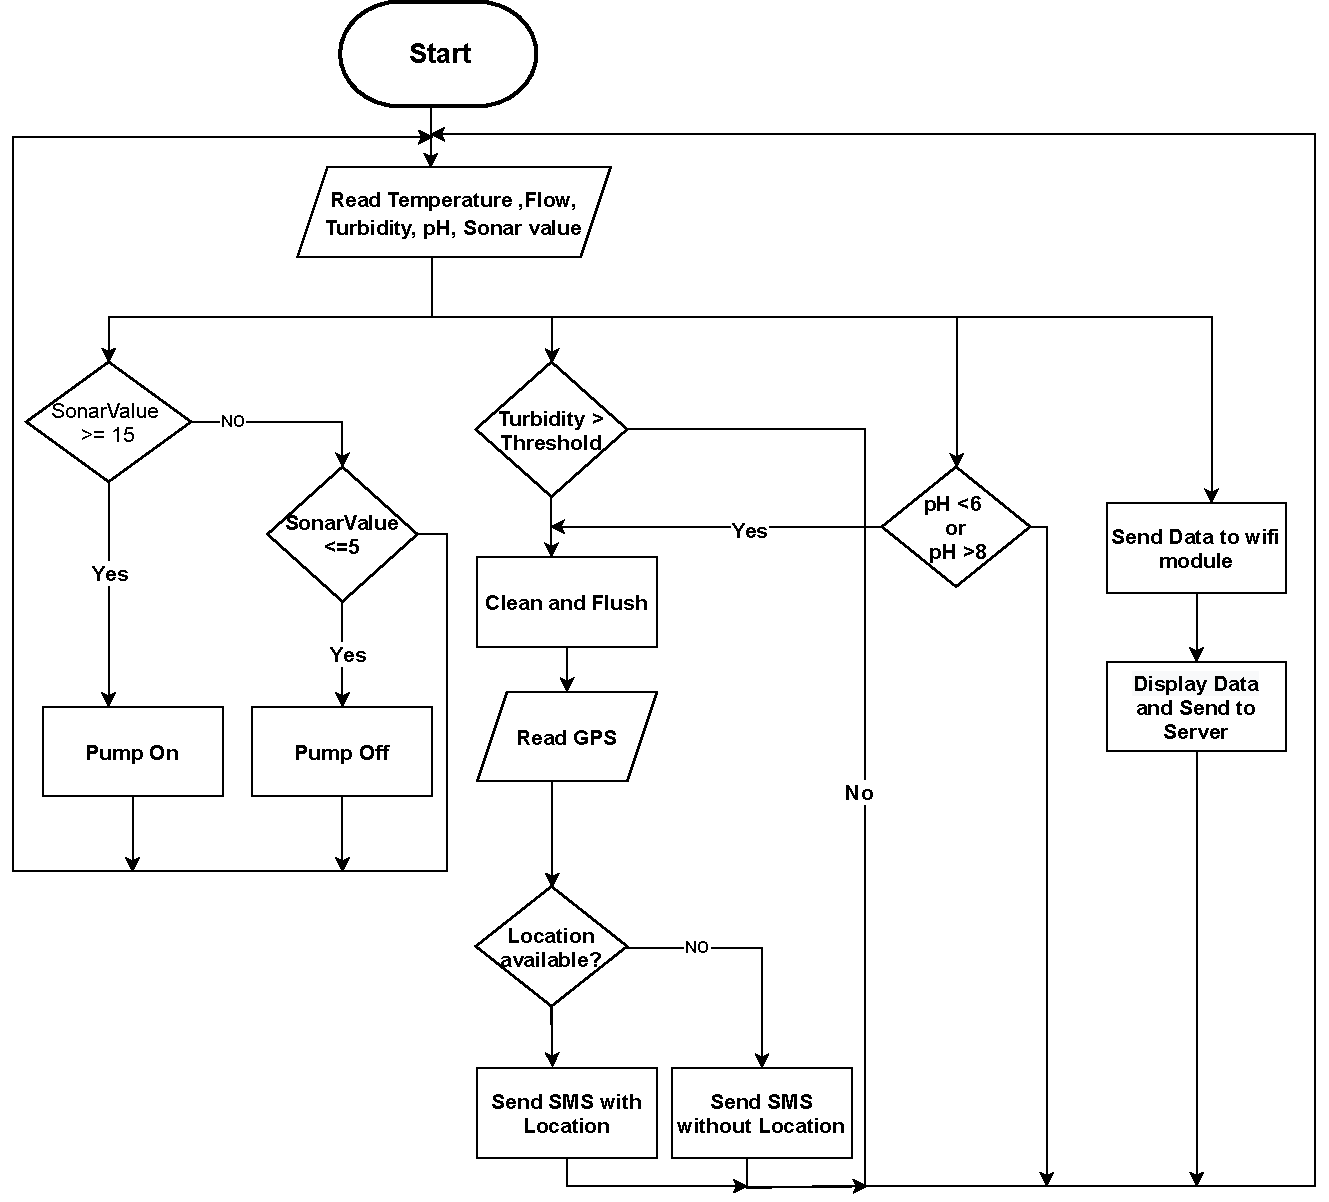
\includegraphics[width=1.0\textwidth]{figures/flow chat.pdf}
\caption{Overall flow chart of proposed system.}
\label{Flow}
\end{figure}
\subsection{Features of This System}
This system has features that are given below:
\begin{itemize}
\item This system can automatically pump water when the tank gets empty.
\item This system can collect the pH level of water.
\item This system can collect dirt level of water.
\item This system can read the water temperature.
\item It can analyse data and find that water is drinkable or not.
\item It can make an early alarm when the water is contaminated.
\item It can clean the water tank and can automatically flush water.
\item It can send tank location to the person in charge when the water gets unusable.
\end{itemize}

\section{Detailed Explanation}
We use different sensors, Google Cloud Storage and an Android app to track the whole device in this IoT based water quality monitoring and control system.
\ref{RealImage} shows the prototype of the proposed model.
In the upcoming section we will describe the schematic diagram, the circuit prototype, and the detailed methodology of the proposed work
\begin{figure}[H]
\centering
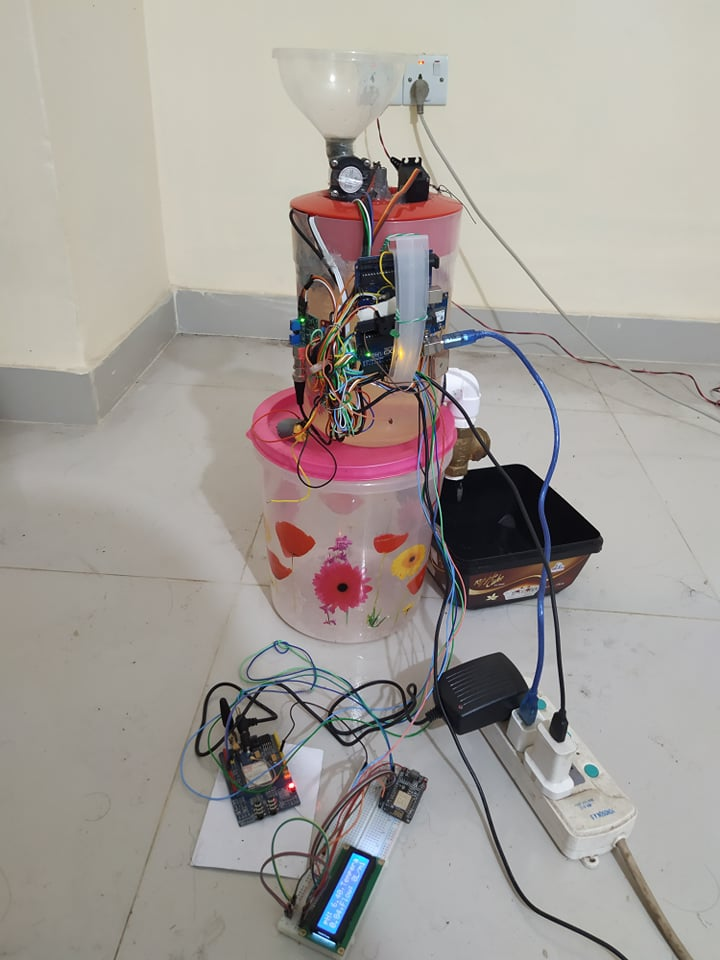
\includegraphics[width=0.9\textwidth]{figures/real_setup.jpg}
\caption{Prototype of the proposed model.}
\label{RealImage}
\end{figure}
%%%%%%%%%%%%%%%%%%%%%%%%%%%%%%%%%%%%%%%%%%%%%%%%
\subsection{Schematic Diagram of the System}
The total schematic diagram of the proposed water quality monitoring and controlling system is given below:

\begin{figure}[H]
\centering
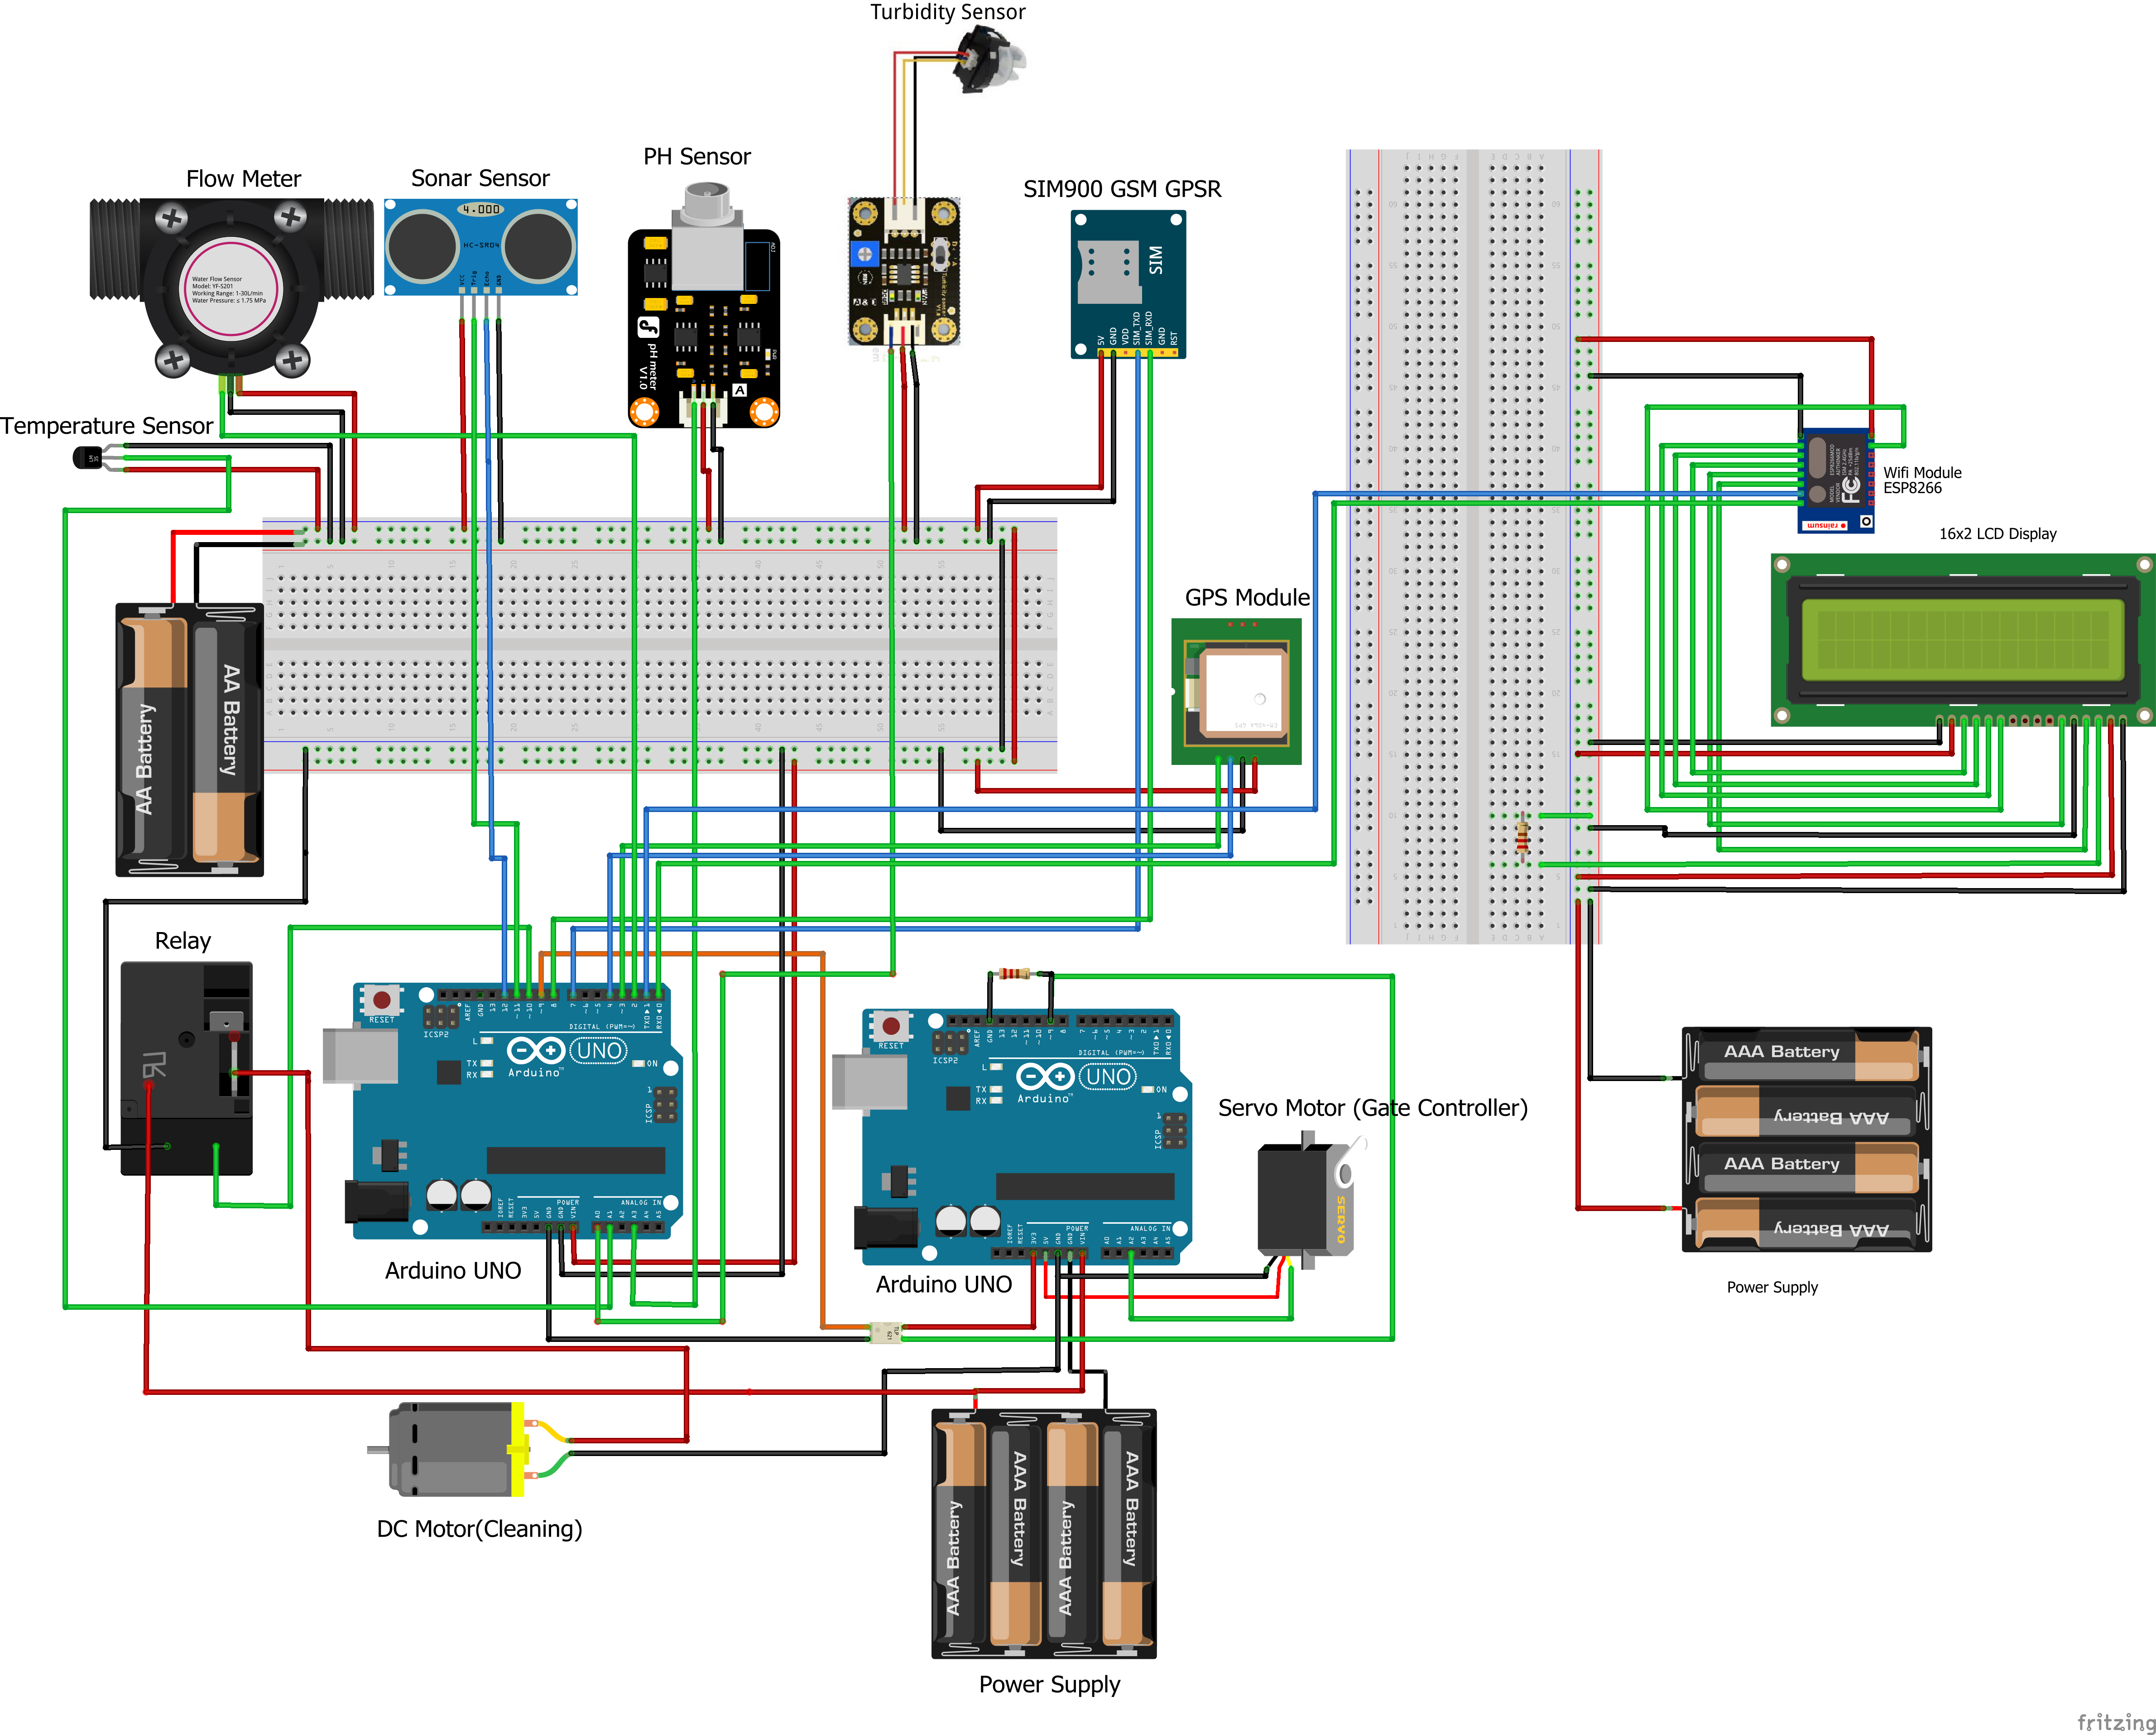
\includegraphics[width=0.9\textwidth]{figures/Final Project Water_bb.png}
\caption{Complete schematic diagram of proposed system.}
\label{SchemaDiagram}
\end{figure}
Initially, we connect the pH sensors and turbidity sensors, flow sensors, temperature sensors with the Arduino UNO. The pH data will be received from the pH sensor, temperature from the temperature sensor, turbidity (How much clean) data will be received from the turbidity sensor, the height of the upper surface of the water will be received from the sonar sensor. From the sonar sensor reading the water volume will be calculated. If the total volume of the tank is V, the area of the tank is A and the height of the upper surface from the top of the tank is h then, water volume is = V-(A*h)
If the upper surface of water exceeds the lower level of the outlet pipe of the tank, then the pump will start automatically. Until the tank gets full with water pump will remain on. when the tank gets full with water it turns the pump off. Also, the turbidity sensor will check the amount of dirt in the water. If the dirt Level exceeds the prefixed limit then it gives an early alarm by buzzer, cleaning motor starts to clean the tank automatically. After a certain time period of cleaning the non-return water gate is opened by a servo motor for flushing the whole water. After flushing the tank servo will close the non-return water gate. So the storage tank is safe. Then GSM module and GPS module are also interfaced with the Arduino UNO. At the time of cleaning, Arduino collects location from the GPS module and using the GSM module the water quality state and location sends to The tank owner number. The controller of the circuit i.e. Arduino UNO, NodeMCU convert analogue data into digital form and send these sensor data to google cloud storage. We created an android application for the Android app to view, track the entire system. To do this, we collected and visualized the data from Google Cloud Storage with the Android application. This application can download the whole data stored in the firebase database.
% \textcolor{red}{MAKE THIS SECTION SHORTER AND Try to explain all the methods explained above separately in the following section}
% \textcolor{blue}{In the upcoming section we are going to explain the detail explanation.}
%%%%%%%%%%%%%%%%%%%%%%%%%%%%%%%%%%%%%%%%%%%%%%%%%%
\subsection{Turning on motor automatically and calculating amount of consumed water}
% \textcolor{red}{change the picture}
In this section we are going to describe how our system turns on the motor automatically and calculate the amount of consumed water which is explained in figure \ref{consumedWater}

\begin{figure}[H]
\centering
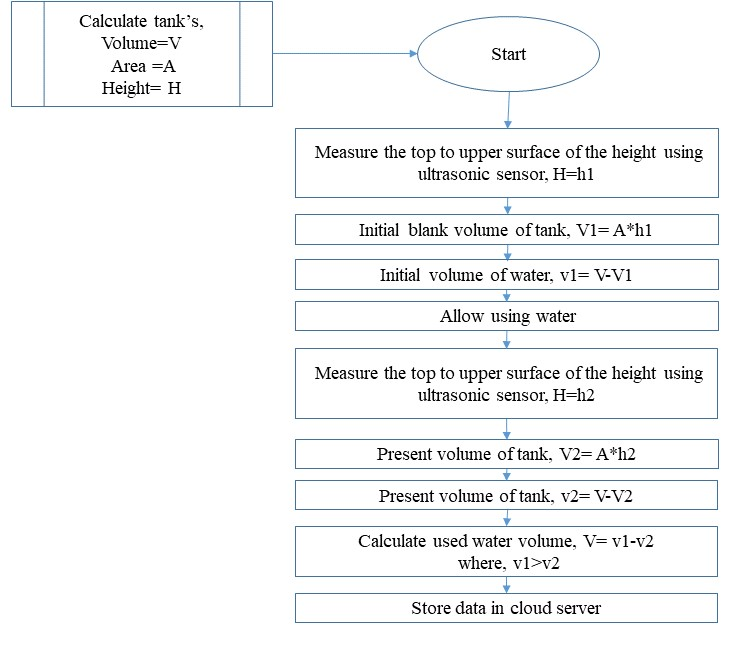
\includegraphics[width=0.5\textwidth]{figures/ConsumedWater.jpg}
\caption{Flow chart of calculating used water}
\label{consumedWater}
\end{figure}
In this project, an ultrasonic sonar sensor is used in the tank. A sonar sensor can calculate the distance of an obstacle. The height of the upper surface of the water will be received from the sonar sensor. From the sonar sensor reading the water volume is calculated. If the total volume of the tank is V, the area of the tank is A and the height of the upper surface from the top of the tank is h then, water volume is = V-(A*h). By reading the volume this system can automatically turn the water pump on or off. Again by subtracting present volume from previous volume we got measured the total volume of used water.. Figure \ref{sonar} shows the connection between the sonar sensor and arduino.
\begin{figure}[H]
\centering
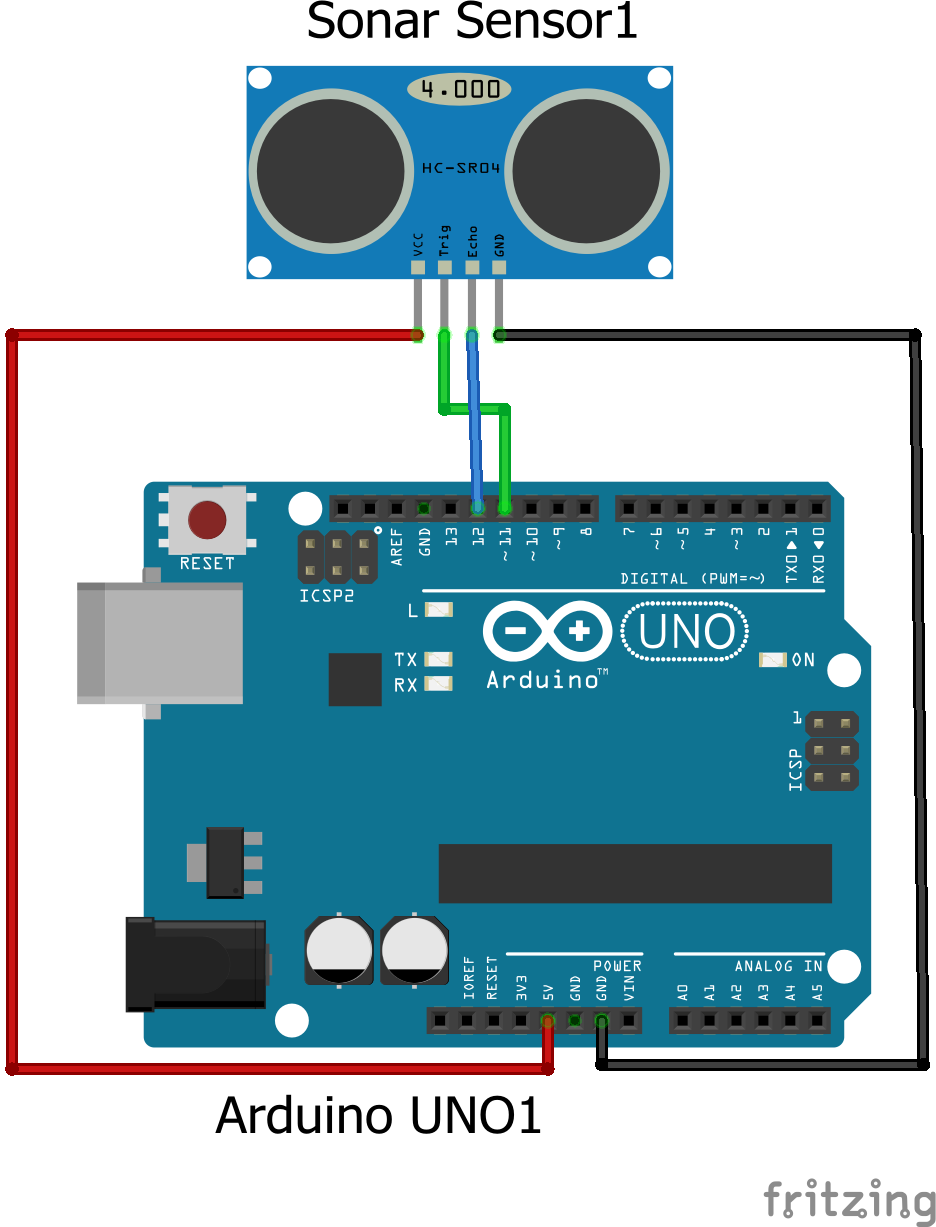
\includegraphics[width=0.5\textwidth]{figures/sonar_bb.png}
\caption{Sonar sensor to Arduino connection}
\label{sonar}
\end{figure}
%%%%%%%%%%%%%%%%%%%%%%%%%%%%%%%%%%%%%%%%%%%%%%%%%%%%
\subsection{Cleaning and flushing the water tank automatically }
This system cleans and flushes the water tank if the  water quality goes under acceptable range. Figure \ref{cleaningFlushing} shows the procedure of cleaning and flushing procedure.
\begin{figure}[H]
\centering
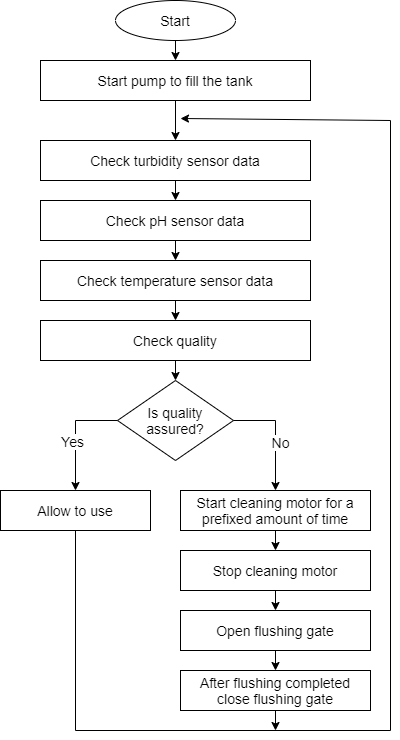
\includegraphics[width=0.8\textwidth]{figures/flow chart of cleaning.png}
\caption{Cleaning and flushing water tank}
\label{cleaningFlushing}
\end{figure}

% \textcolor{red}{WRITE DOWN THE PARAMETERS YOU HAVE CONSIDERED FOR YOUR OWN EXPERIMENT}
% \textcolor{blue}{CHECK IF THE STEPS ARE OK OR NOT}
To measure the quality of water good or bad first we calibrated the sensors. After then we read sensors data of water. We compared the sensors value to the standard value of water. The standard range value of pure water according to WHO is given below. If data remains in this range we coincided as good water. And if data exceeds the range we coincided water as bad water.
\begin{table}[H]
\centering
\caption{Quality parameter value range of pure water provided by WHO}
\begin{tabular}{|c|c|c|}
\hline
\textbf{Sensor}    & \textbf{Value range} & \textbf{Unit} \\ \hline
\textbf{pH}        & \textbf{6.5-8.5}     & \textbf{pH}   \\ \hline
\textbf{Turbidity} & \textbf{5-10}        & \textbf{NTU}  \\ \hline
\end{tabular}
\end{table}

The system follows the following steps to clean and flush the water tank.
\begin{itemize}
    \item Check quality of water
    \item Clean the tank
    \item Flush the water
    \item Fill the tank again
\end{itemize}
\subsubsection{Checking the quality of the water}
To assure quality the system checks temperature, pH value and turbidity value
\subsubsection*{Collecting Temperature of Water}
In our system DS18B20 waterproof temperature sensor is used inside the tank. Arduino collects supplying voltage from the temperature sensor and calculates water temperature both in Celsius and Fahrenheit.Figure \ref{TempSensor} shows the connection between the temperature sensor and arduino.
\begin{figure}[H]
\centering
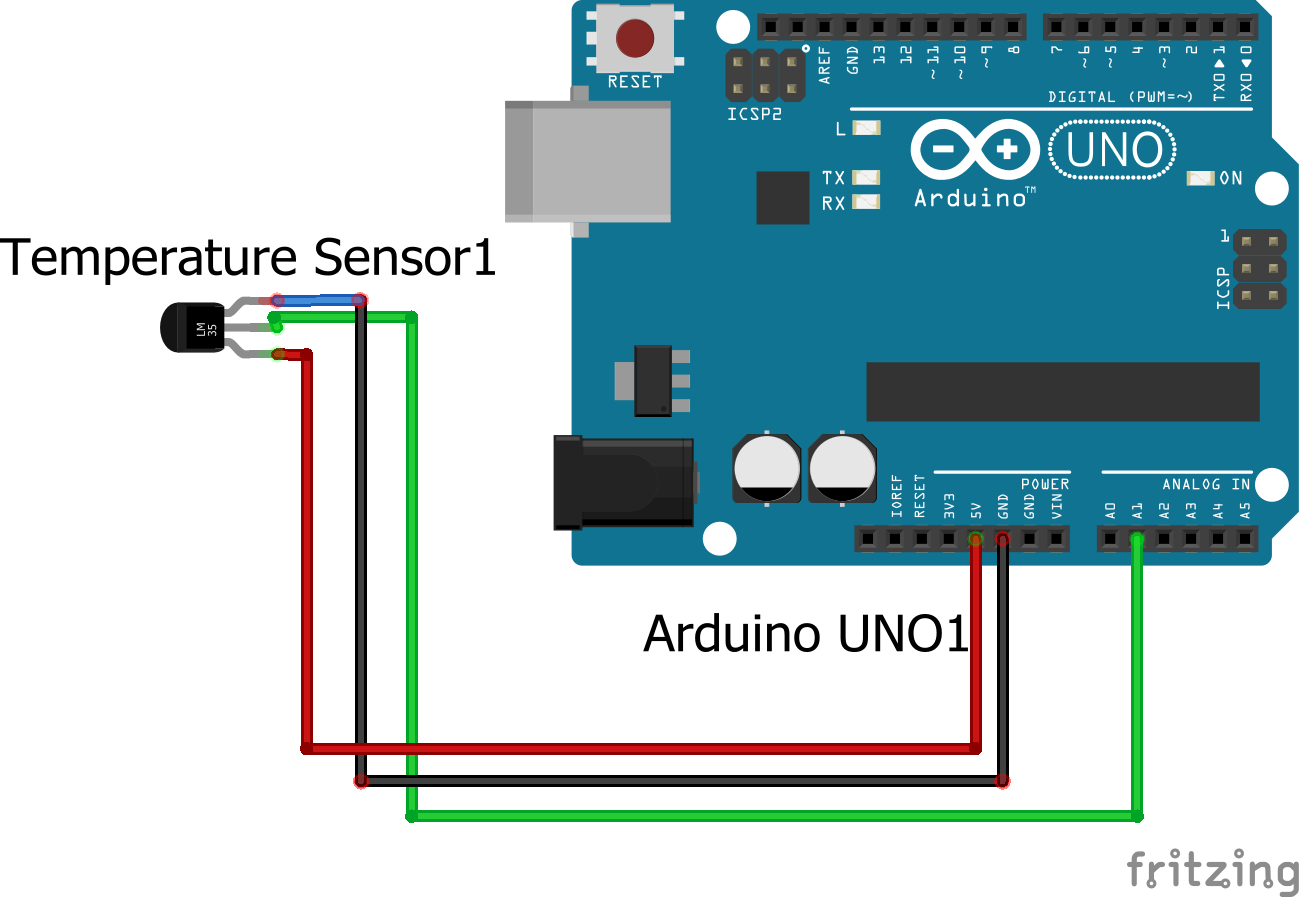
\includegraphics[width=0.5\textwidth]{figures/Temperature_bb.png}
\caption{Temperature sensor to Arduino connection}
\label{TempSensor}
\end{figure}
\subsubsection*{Collecting Turbidity Value}
In our system turbidity sensor is used to getting the dirt level of water. Turbidity sensor supply electrical voltage to Arduino. Arduino calculates NTU from those voltages.

\begin{figure}[H]
\centering
\subfloat[Turbidity sensor to Arduino connection]{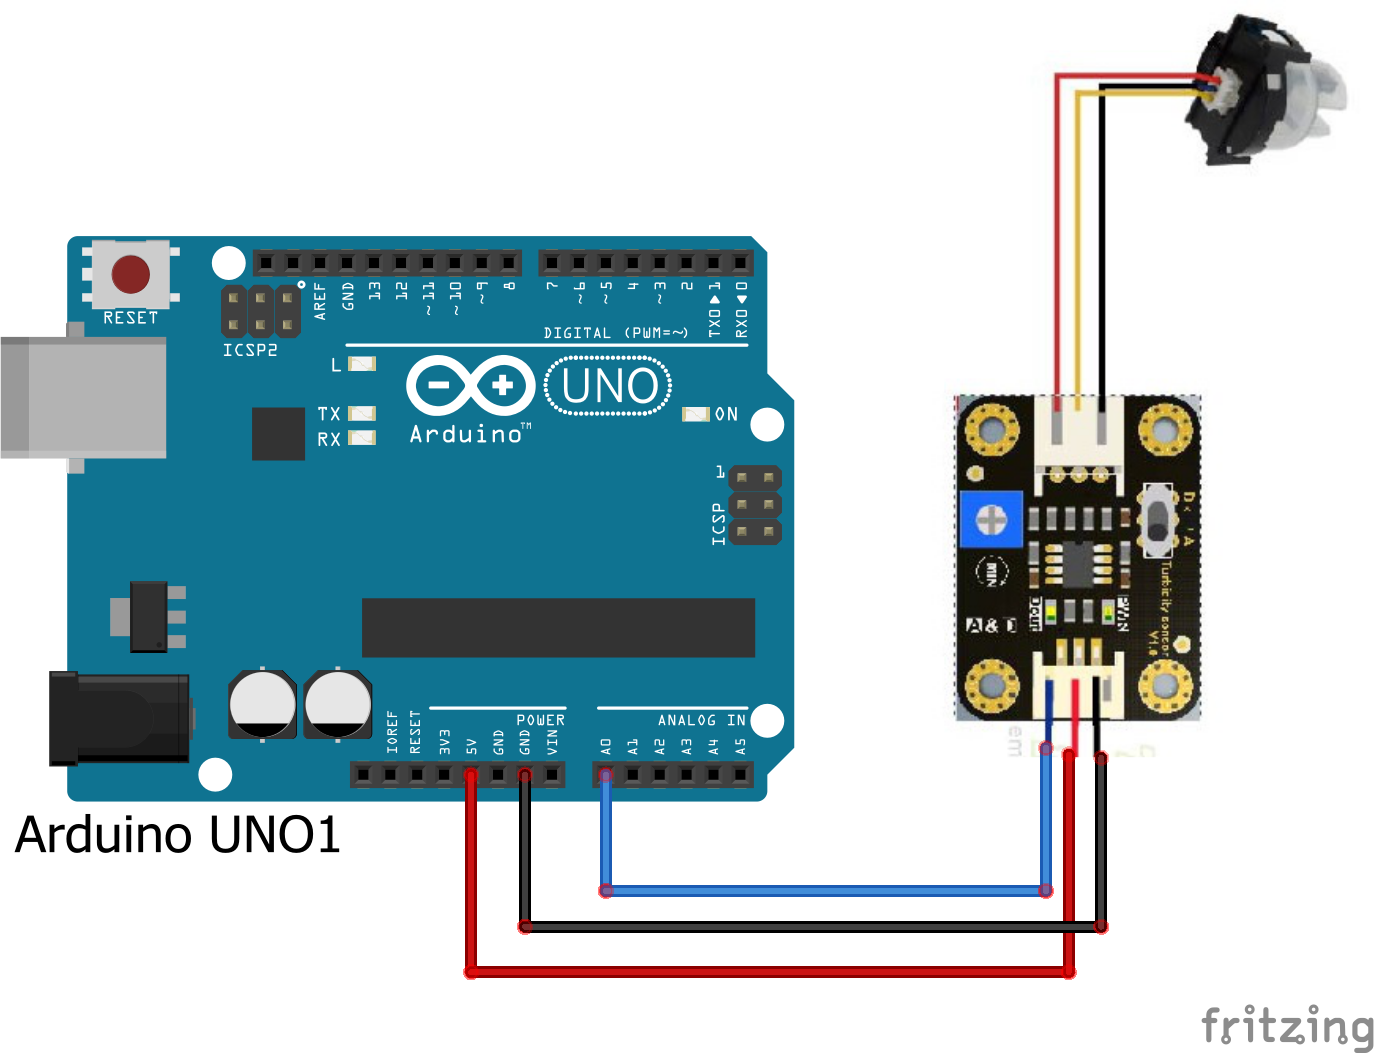
\includegraphics[width = 0.3\textwidth]{figures/tarbidity_bb.png}} 
\hspace{2cm}
\subfloat[NTU vs Voltage ]{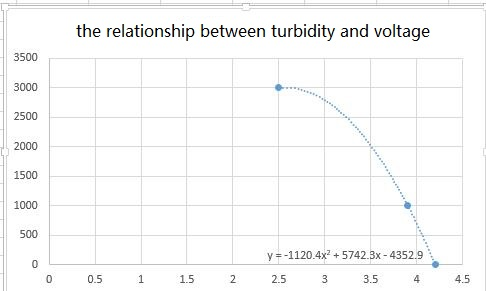
\includegraphics[width = 0.3\textwidth]{figures/turvsvoltage.jpg}}

\caption{Turbidity value calculation}
\end{figure}
\subsubsection*{Collecting pH Value}
in this section, we will discuss collecting the pH value of water.
pH meter can read 0-14 range of value. In our system, it is placed inside the tank. as it reads the real-time acidity value. It is connected to Arduino, based on the supply voltage Arduino calculates the pH value. Figure \ref{pHandBB} shows the connection of pH sensor with arduino.
\begin{figure}[H]
\centering
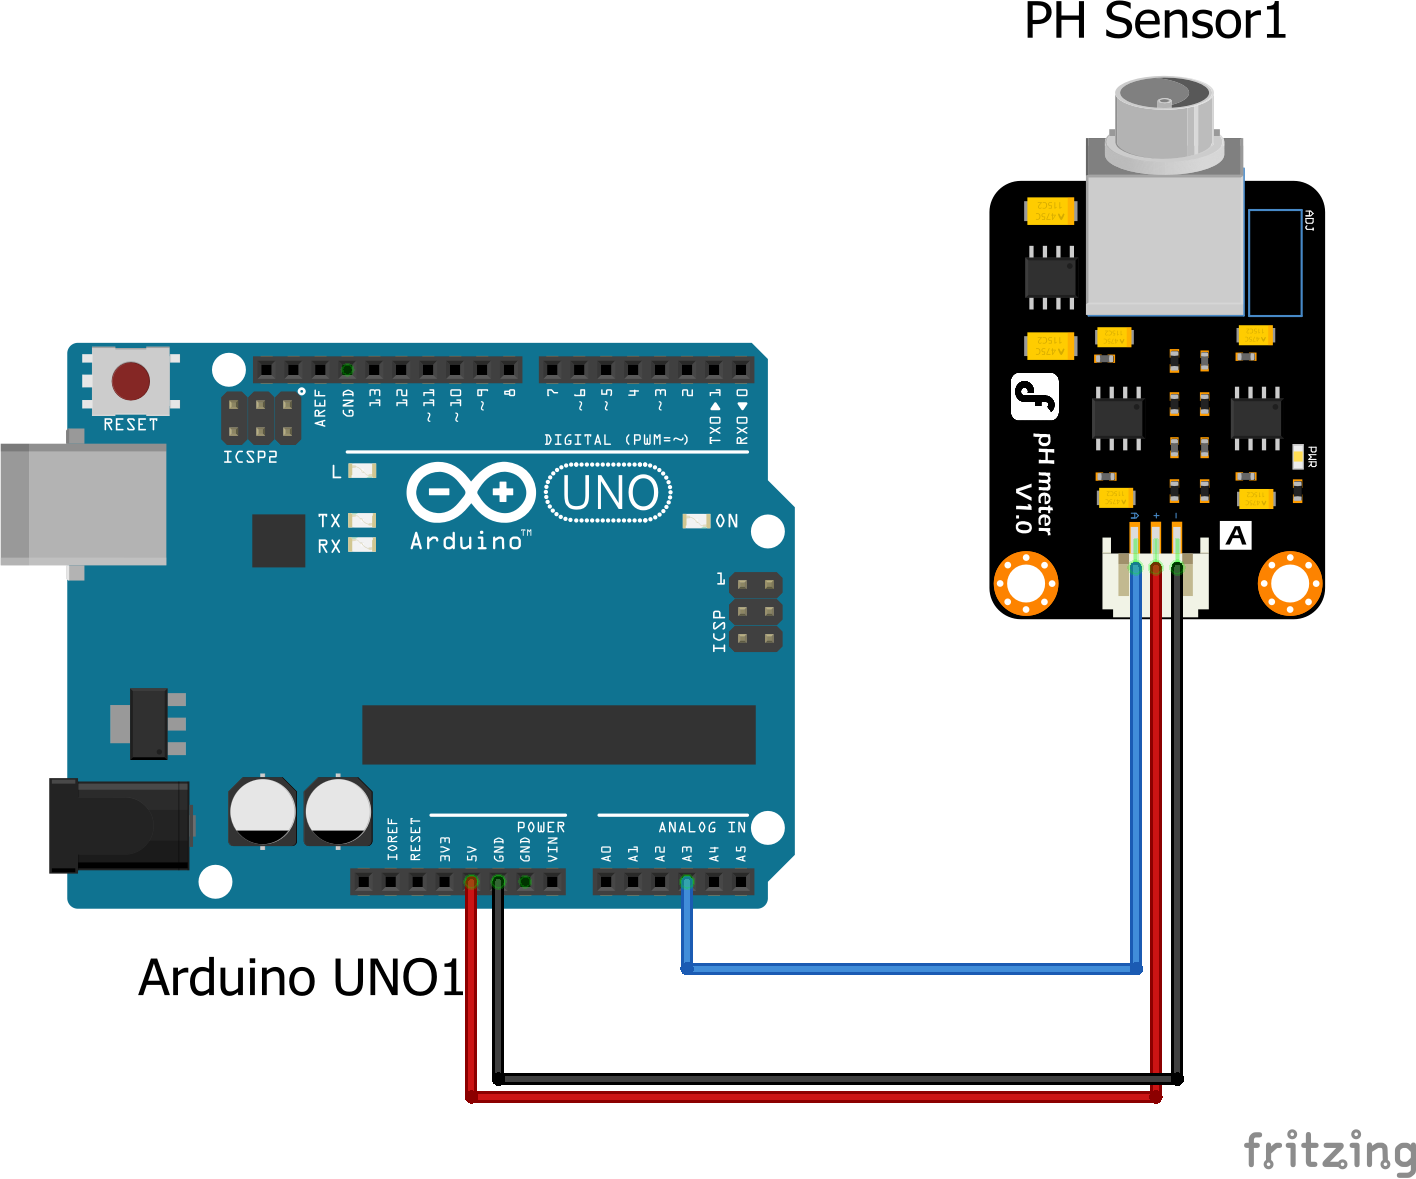
\includegraphics[width=0.5\textwidth]{figures/PH_bb.png}
\caption{pH sensor to Arduino connection}
\label{pHandBB}
\end{figure}
pH value of water can be 0-14 range. Neutral water has pH of 7. If the pH value decreases it becomes acidic and if pH value increases it becomes alkaline. we According to WHO we consider drinking water pH>6.5 and pH<8.5 .if pH crosses this, limit we recognized it as bad water. 
% \subsubsection*{Assuring quality} \textcolor{red}{EXPLAIN WHY YOU ARE SAYING THAT THE WATER QUALITY IS GOOD FOR EXAMPLE IF PH VALUE IS < 3.5 THE SYSTEM WILL RECOGNIZE THAT THE WATER QUALITY IS GOOD}
\subsubsection{Cleaning the Tank}
By analysing sensor data when the system detects that water gets dirty it starts the cleaning motor to clean the inner layer of the tank. A nylon brush is used to clean. This motor has high torque and to drive the high current is needed. As this type of motor consumes high power electricity. Thus Arduino cannot supply so much power, the motor is switched by a relay device. A relay switch is an electromagnetic device that can drive high power electricity switched by low power electricity. Figure \ref{DCMotor} shows the connection between the DC motor and arduino.
\begin{figure}[H]
\centering
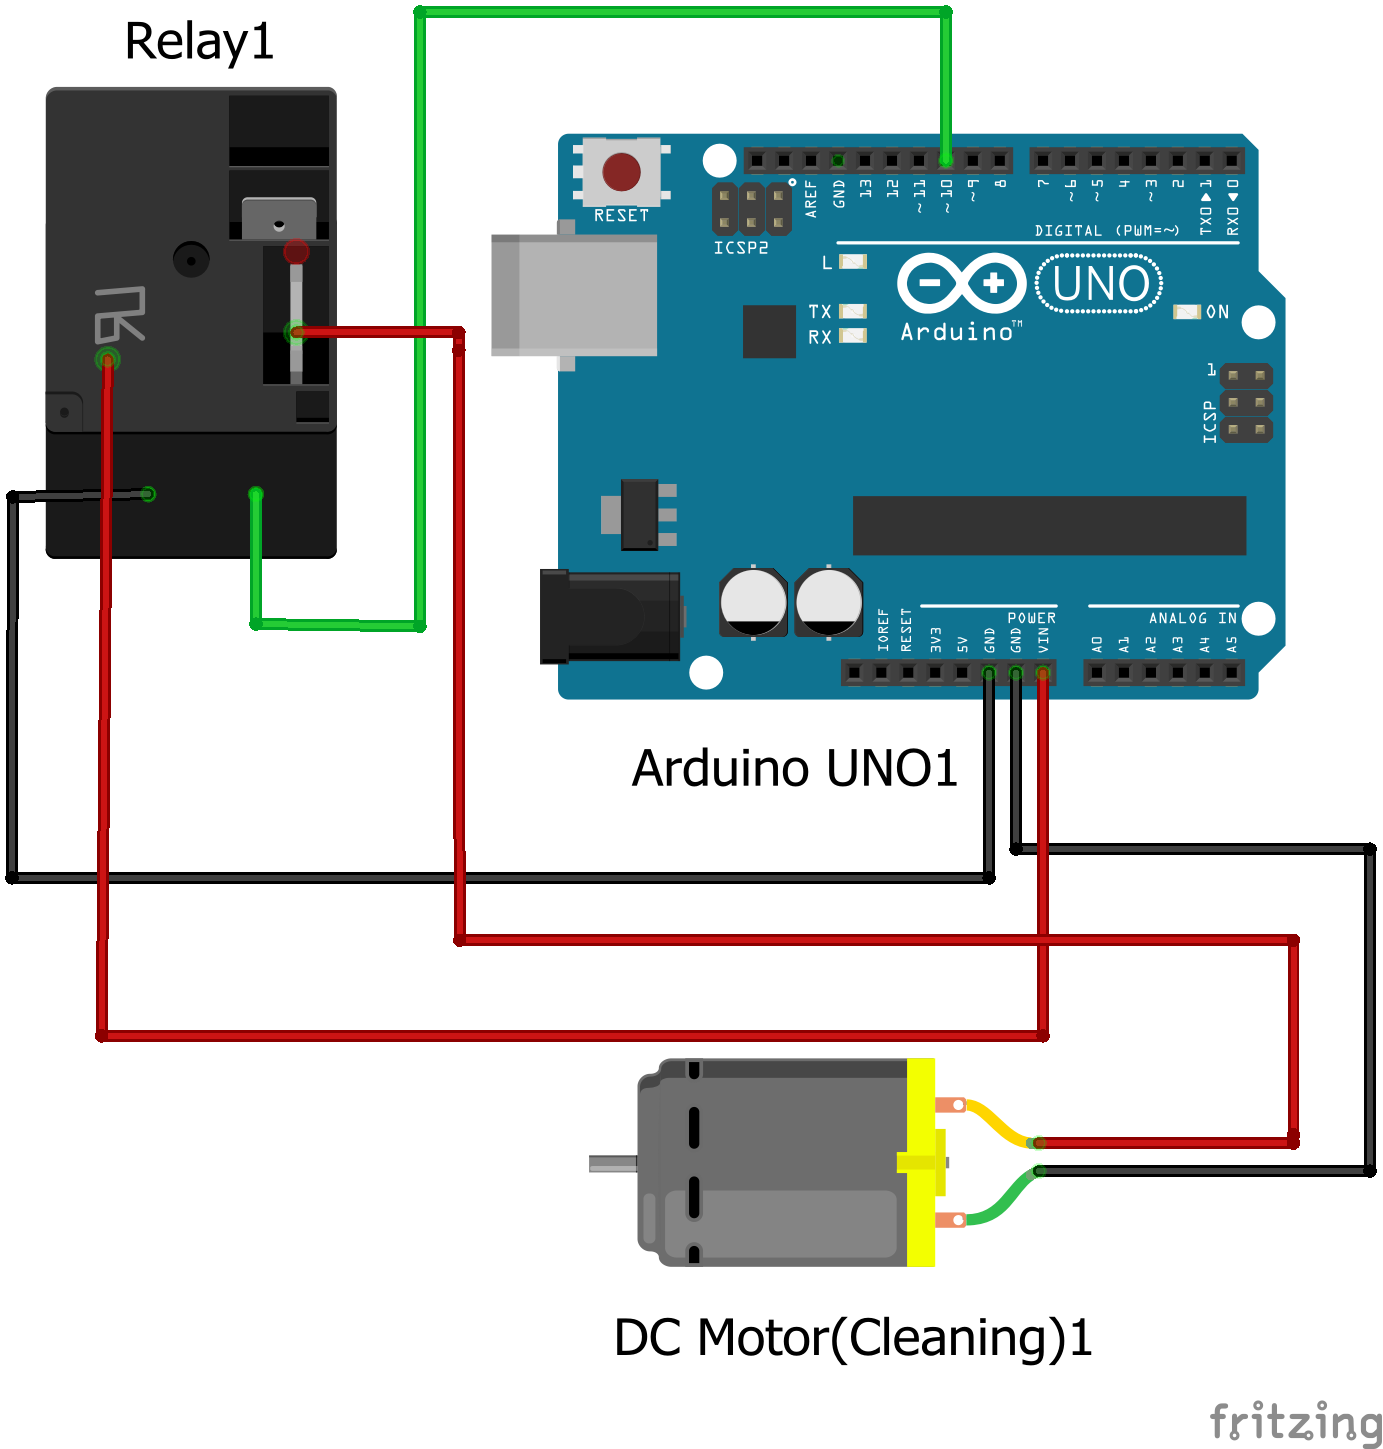
\includegraphics[width=0.5\textwidth]{figures/Motor_bb.png}
\caption{DC cleaning motor to Arduino connection}
\label{DCMotor}
\end{figure}
\subsubsection{Flushing the water tank}
By switching servo motor using optocoupler and arduino the syste, flush the water tank.
A Servo motor is used to open the gate when it needs to flush water. But servo motor needs a data signal to rotates at a fixed angle. In this project many sensors and computation is used so for fluctuation of electricity sometimes servo behaved wrongly so we needed to switch it optically. we used an optocoupler to switch to another Arduino. In the following diagram, it is shown. when the second Arduino gets a switching pulse it sends rotating signals to the servo motor and the servo motor starts to rotate for opening or closing water flushing gate.

\begin{figure}[H]
\centering
\subfloat[Arduino connection to Arduino with optocupler]{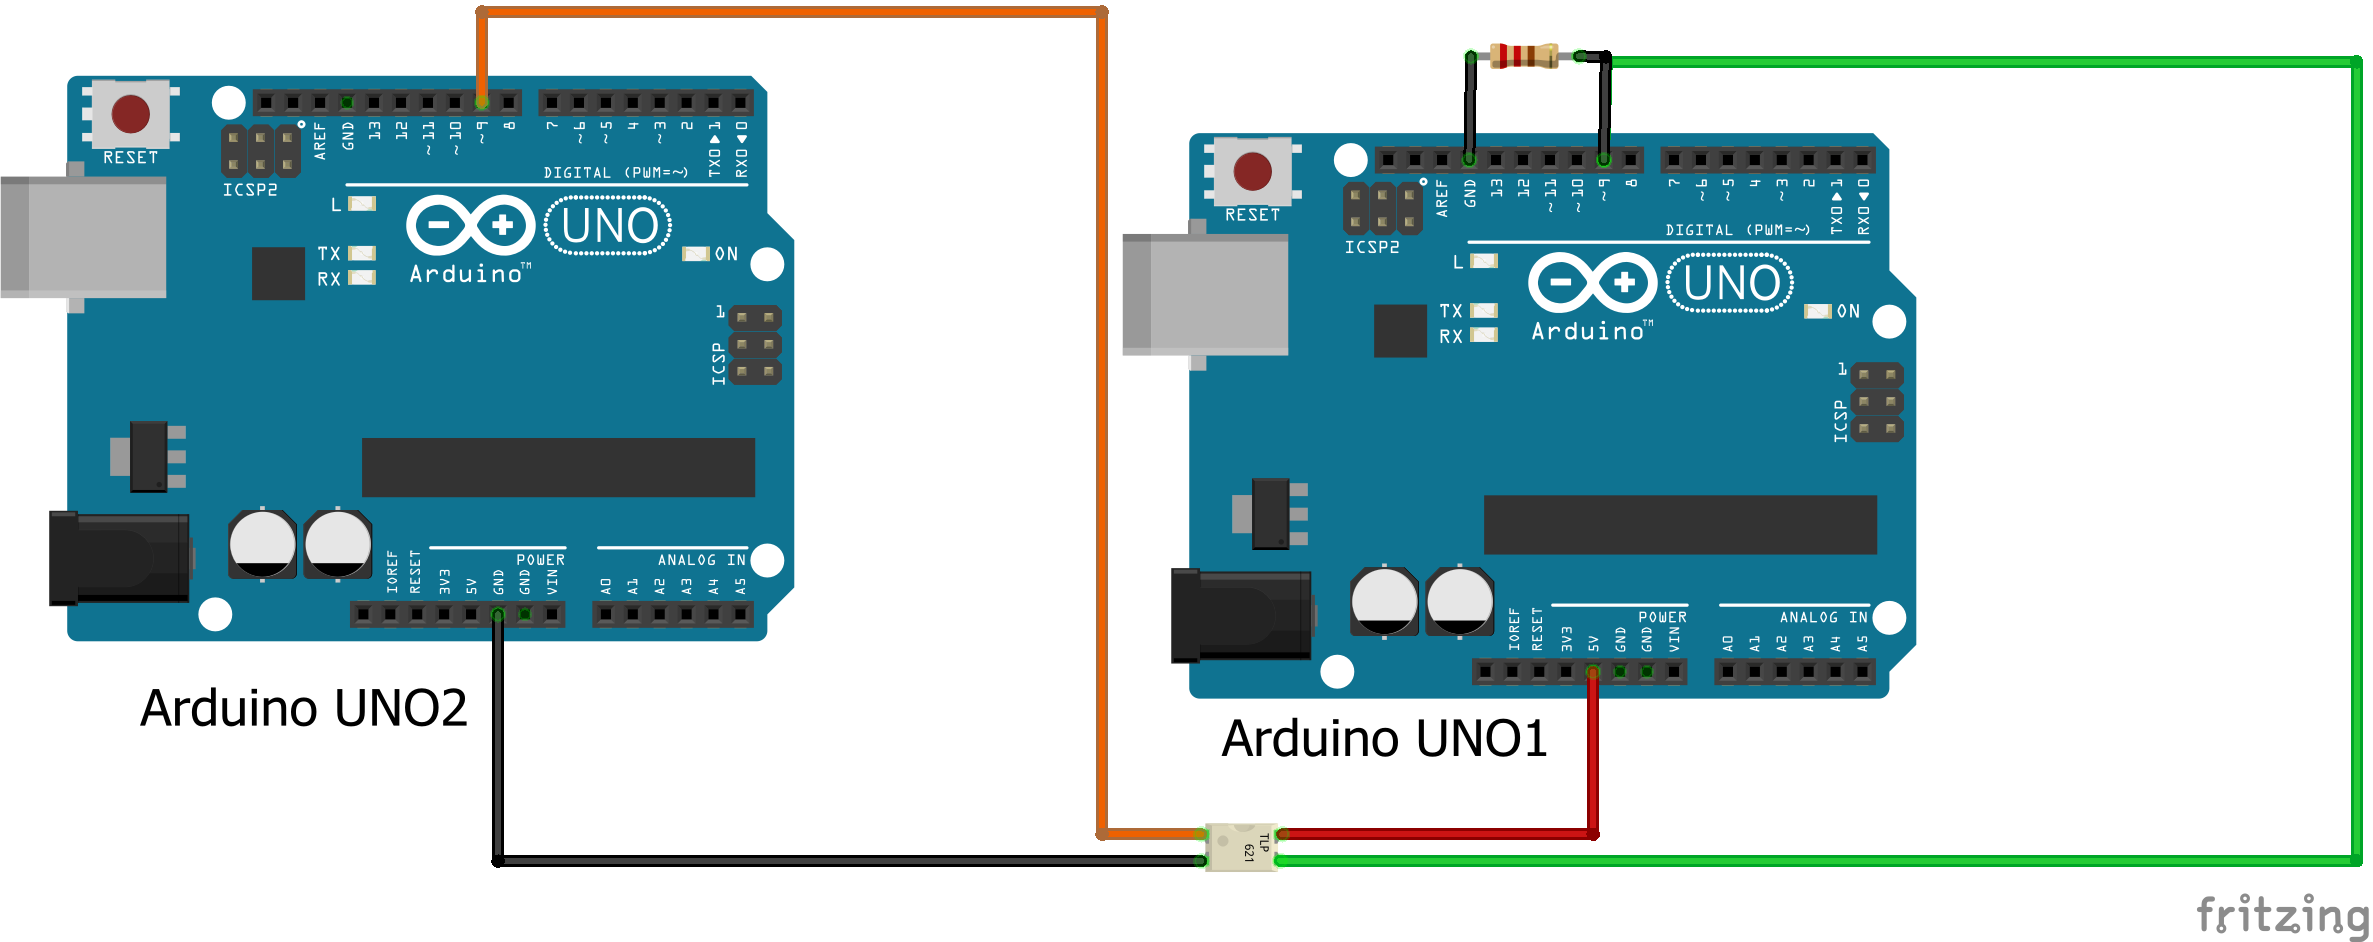
\includegraphics[width = 0.35\textwidth]{figures/arduinoTOarduino_bb.png}} 
\hspace{2cm}
\subfloat[Servo to Arduino connection]{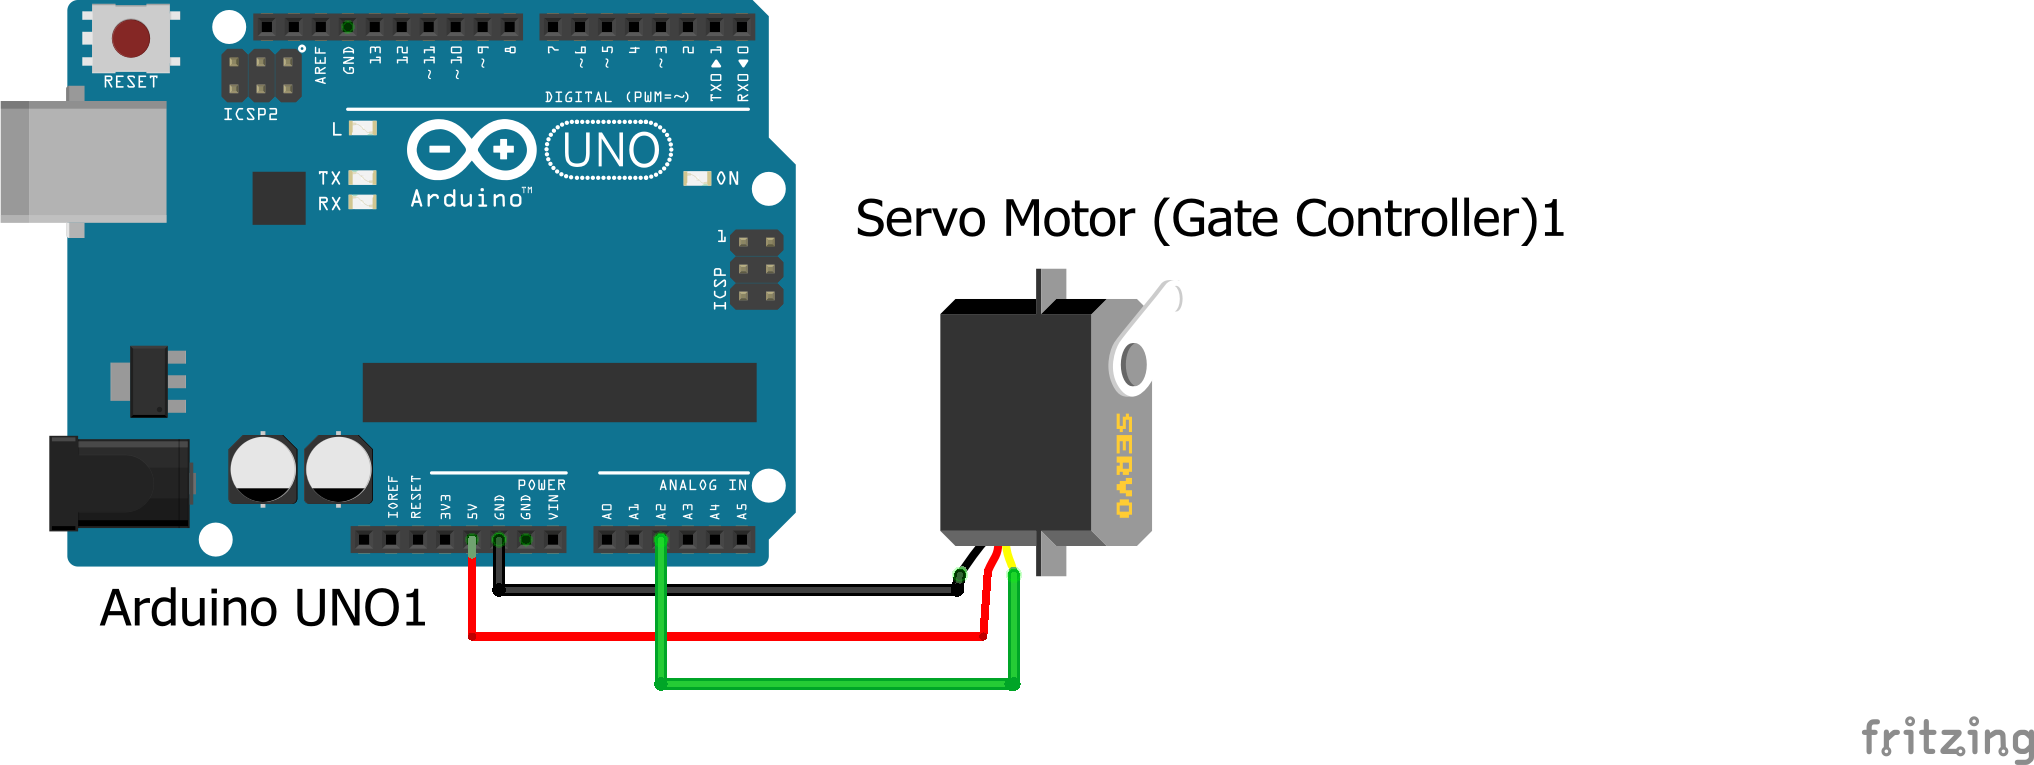
\includegraphics[width = 0.35\textwidth]{figures/servo_bb.png}}
\caption{Driving servo motor}
\end{figure}
%%%%%%%%%%%%%%%%%%%%%%%%%%%%%%%%%%%%%%%%%%%%%%%%%%%%
\subsection{Sending a warning message with location to the in charge   if water pollution occurs.
}
% \textcolor{red}{TRY  TO PROVIDE A FLOW CHART SHOWING THE FEATURE OF THE ANDROID APP.figure 3.15,3.16,3.17 WILL BE IN IMPLEMENTATION SECTION.. I AM DOING THIS>... YOU NEED TO PREPARE A FLOW OR BLOCK DIAGRAM REPRESENTING SENDING ALERT MESSAGE}
% \subsubsection*{Checking data}
After collecting all sensors data it checks the quality. If quality is not good then it sends SMS with GSM module after trying to collect location info from GPS module.  Figure \ref{smsflow1} shows the flow chart of sending alert SMS.
\begin{figure}[H]
\centering
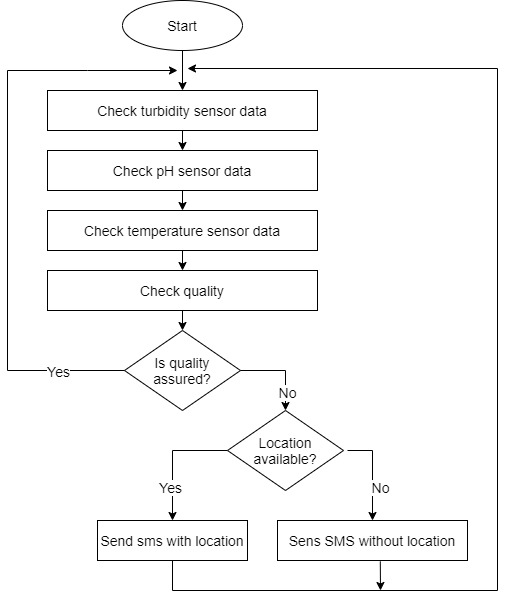
\includegraphics[width=0.5\textwidth]{figures/flow chart of sendibg sms.jpg}
\caption{SMS sending flow chart}
\label{smsflow1}
\end{figure}

\subsubsection*{Collecting GPS Location}
We used a GPS module in our system to get the tank location. When the water gets unacceptable to use the location will be sent to the responsible person. Figure \ref{GpsModule1} shows the connection between the Gps module and Arduino.
\begin{figure}[H]
\centering
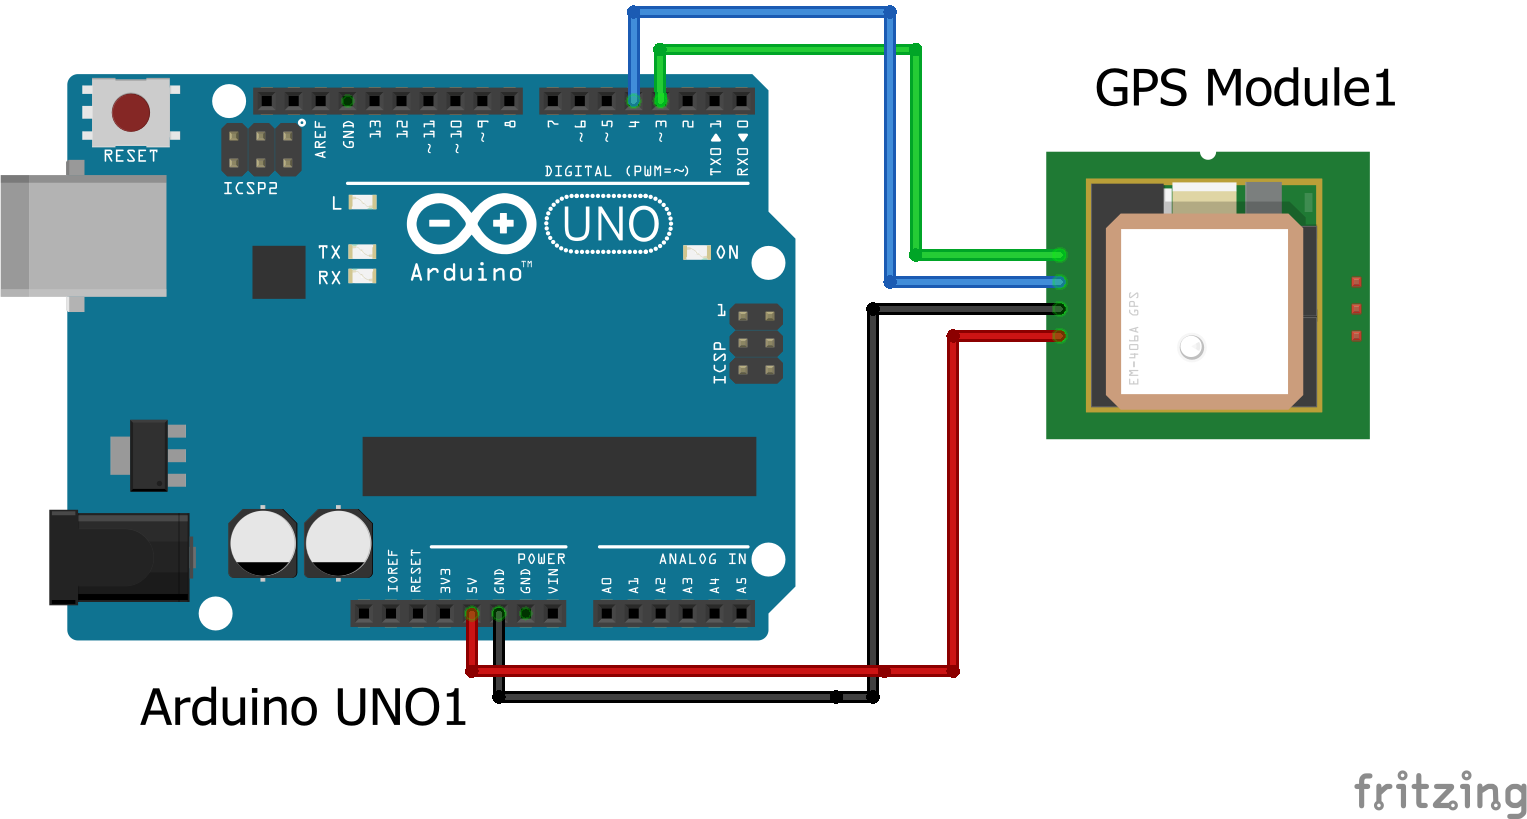
\includegraphics[width=0.5\textwidth]{figures/gps_bb.png}
\caption{GPS module to Arduino connection}
\label{GpsModule1}
\end{figure}



\subsubsection*{Sending SMS}
We used GSM GPRS module to send location and notification message to respective person when water gets dirty.Figure \ref{GSMMod} shows the connection between the sonar sensor and Arduino.

\begin{figure}[H]
\centering
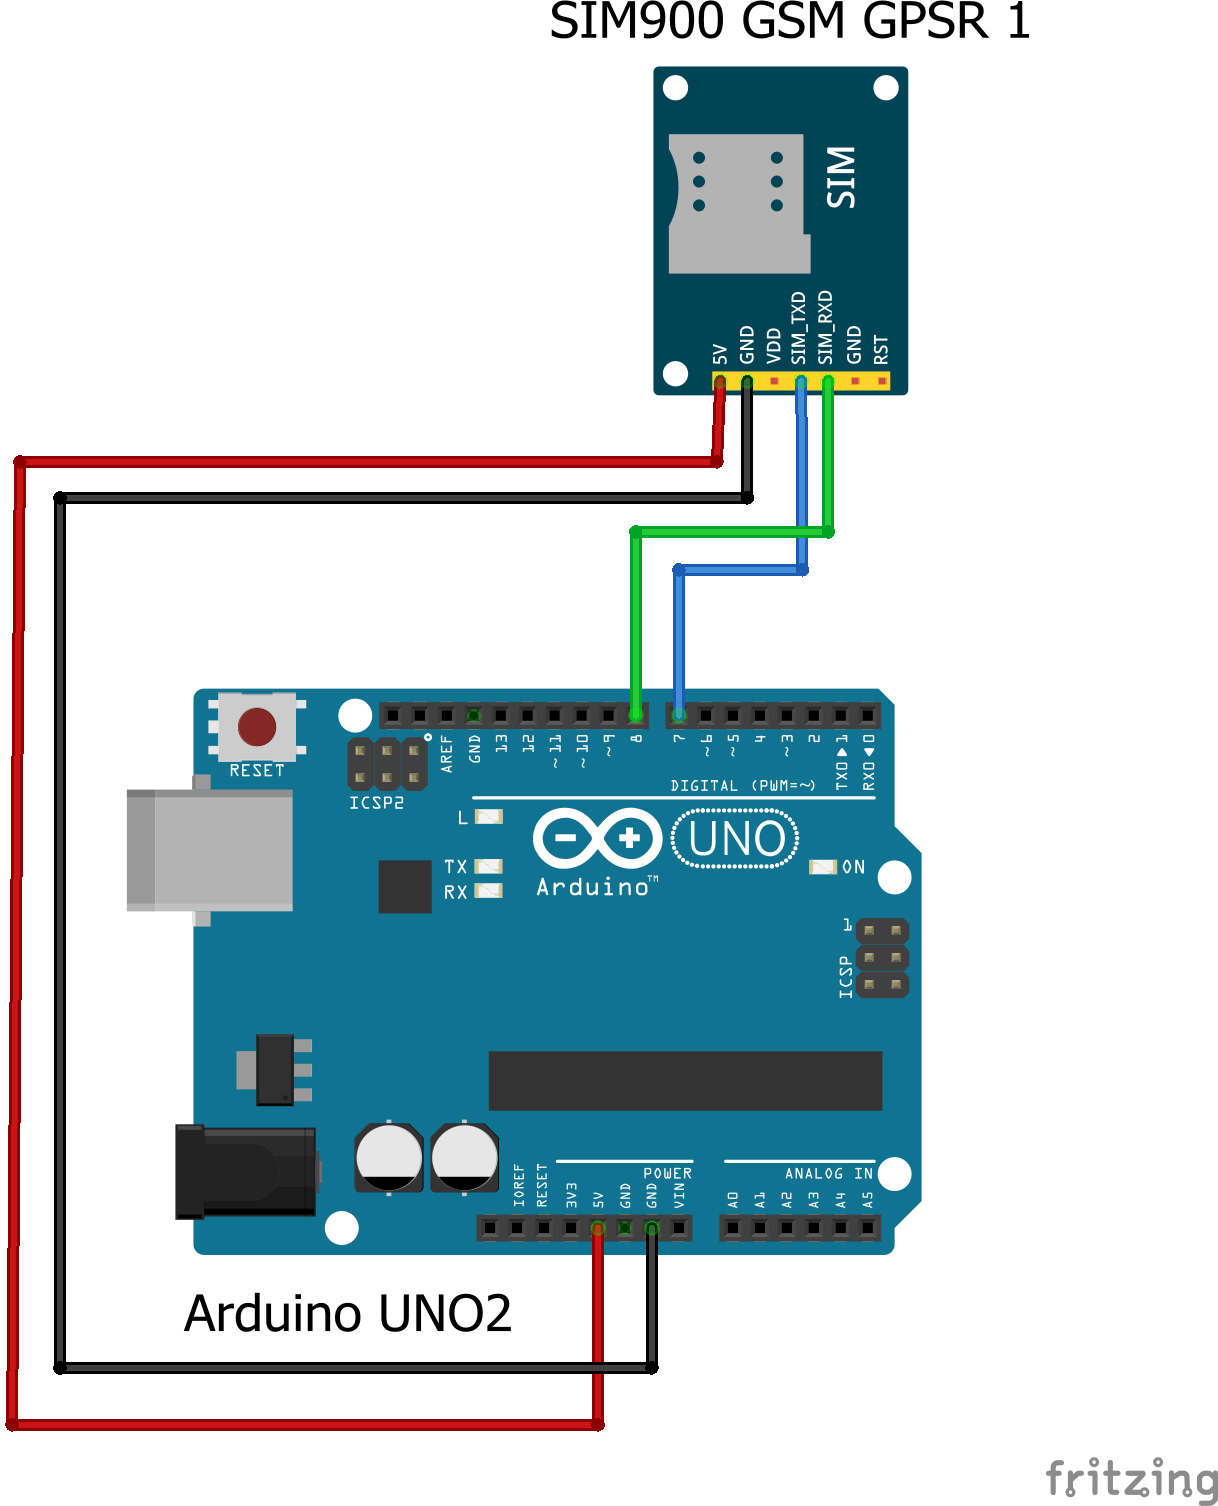
\includegraphics[width=0.5\textwidth]{figures/sim_bb.png}
\caption{GSM module to Arduino connection}
\label{GSMMod}
\end{figure}

\subsubsection*{Android Application as Output Interface}
We developed an android interface to visualize the data. Firebase realtime database SDK is provided by Google to make the application accessible to the database. We used that SDK as API in the application. This application is very easy to use and simple to understand. It has two interfaces in the first interface displays the latest condition of the water. We see the pH, Temperature, Turbidity, Flow, Used, volume value in the app interface. 
\begin{figure}[H]
\centering
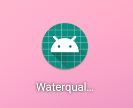
\includegraphics[width=0.3\textwidth]{figures/application_icon.JPG}
\caption{Android application Icon}
\label{ICON}
\end{figure}

Updated data image is given below:

\begin{figure}[H]
\centering
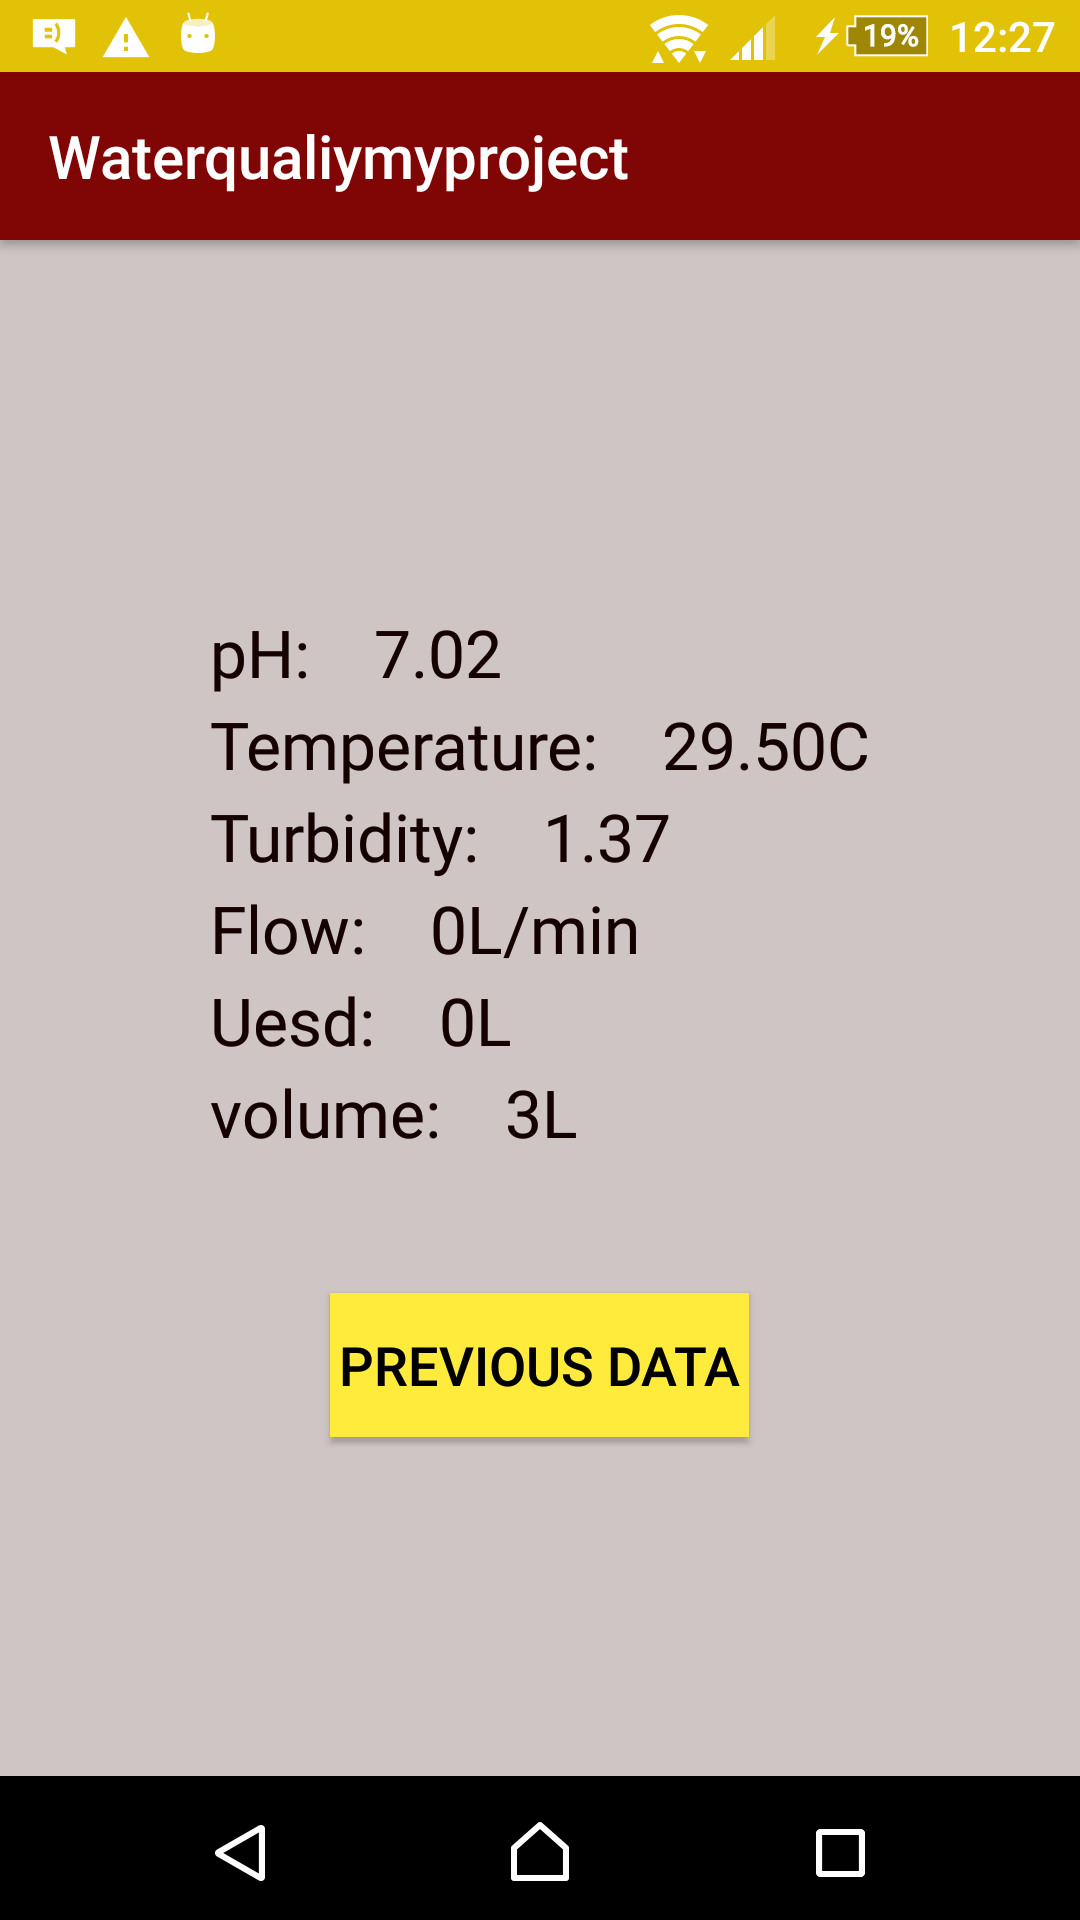
\includegraphics[width=0.5\textwidth]{figures/171806466_876139099631416_6409685255133294248_n.png}
\caption{Android app updated data.}
\label{UpdateAndroid}
\end{figure}

In the app interface, a button called "PREVIOUS DATA" is added. By pressing this button, we can go to second interface which shows us all the data from beginning to end. 

"Previous data" interface image is given below:
\begin{figure}[H]
\centering
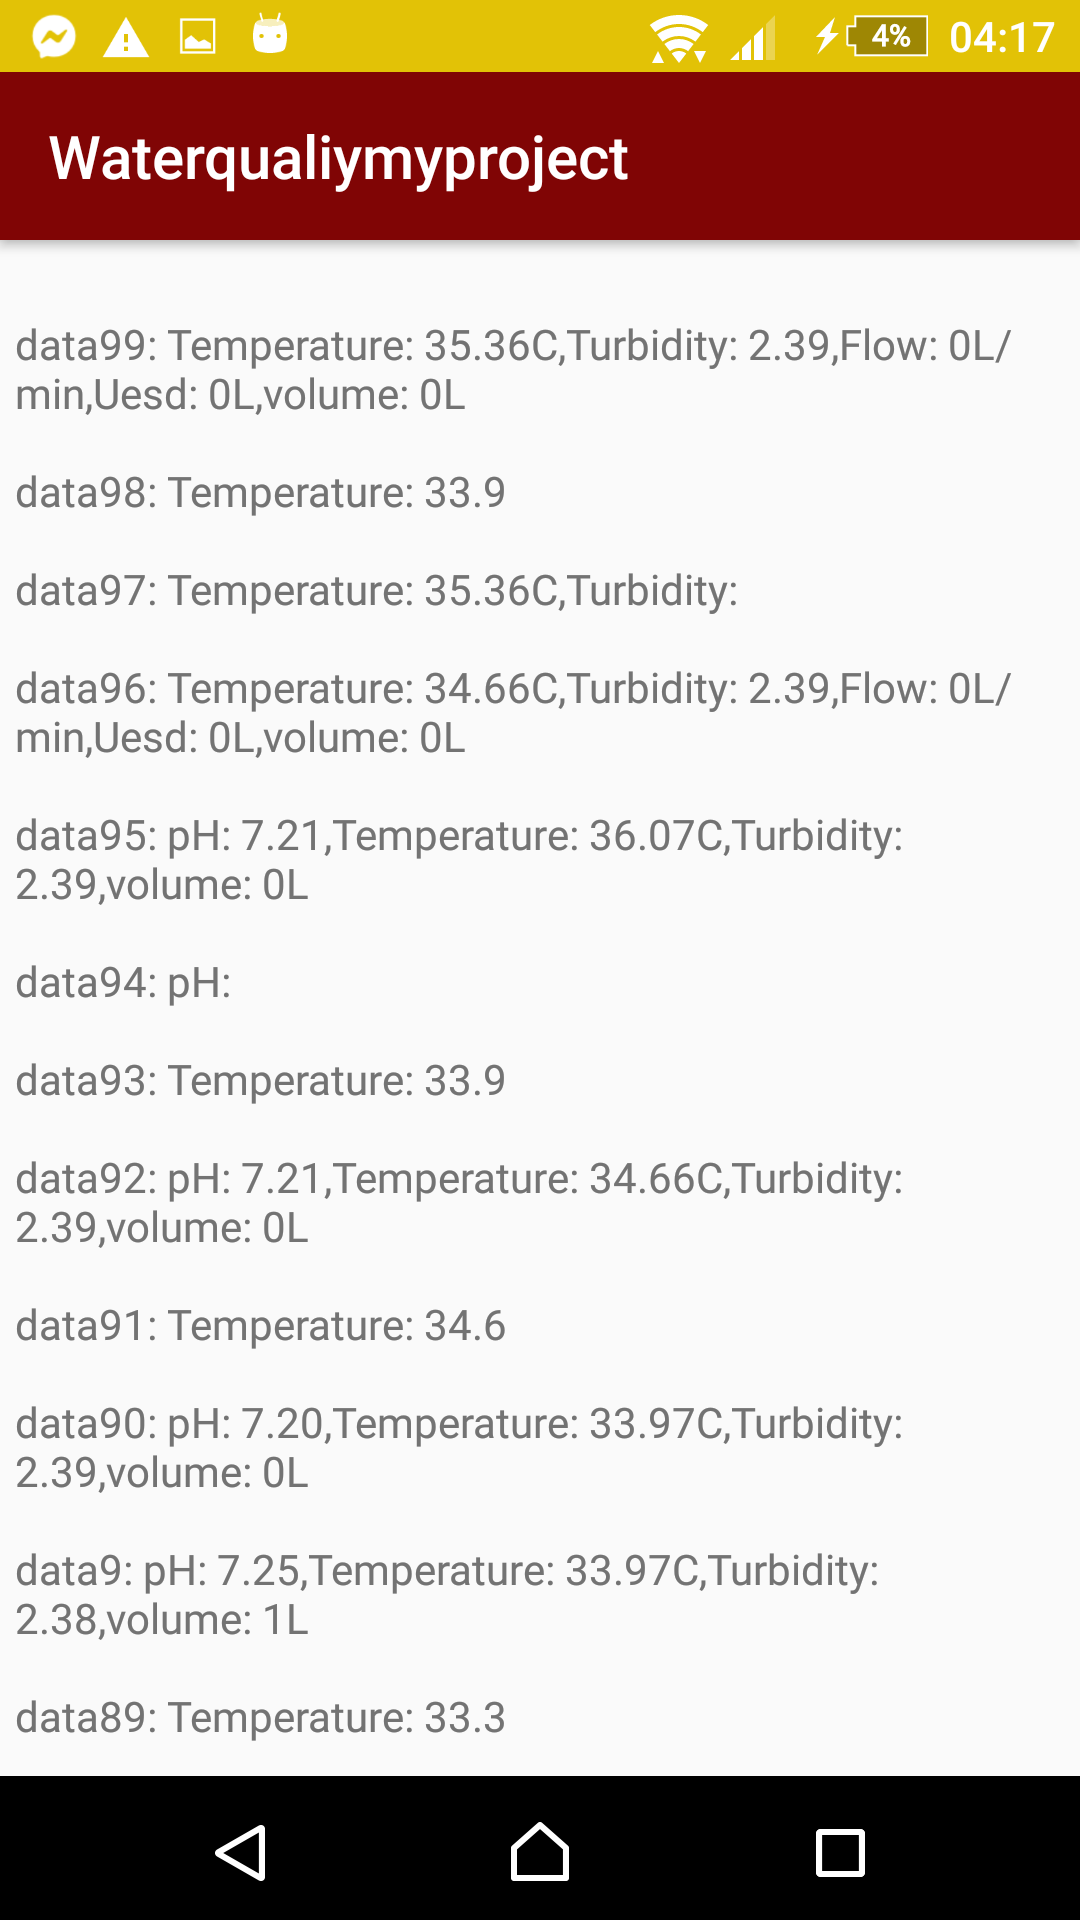
\includegraphics[width=0.5\textwidth]{figures/173292020_499998037660544_1209567427091880898_n.png}
\caption{Android app previous data.}
\label{PreviousDataAndroid}
\end{figure}
\subsubsection*{Incoming SMS with Location}
We included the SMS sending process in our system. when the water gets dirty, it sends SMS with location to respective person as an alert.
\begin{figure}[H]
\centering

\includegraphics[width=0.4\textwidth]{figures/sms.jpg}
\caption{Alerting message with tank location}
\label{AlertMessage}
\end{figure}

%%%%%%%%%%%%%%%%%%%%%%%%%%%%%%%%%%%%%%%%%%%%%
%%%%%%%%%%%%%%%%%%%%%%%%%%%%%%%%%%%%%%%%%%%%%%%%%%%%
\subsection{Showing water flow rate on LCD display}
\subsubsection*{Collecting Flow Rate of Water}
In our system flow meter used at the inlet pipe thus the rate of entering the water can be measured. Arduino collects generated voltage from the flow sensor and calculates the rate of passing water from this voltage.
Figure \ref{FlowSensor} shows the connection between the flow sensor and arduino.
\begin{figure}[H]
\centering
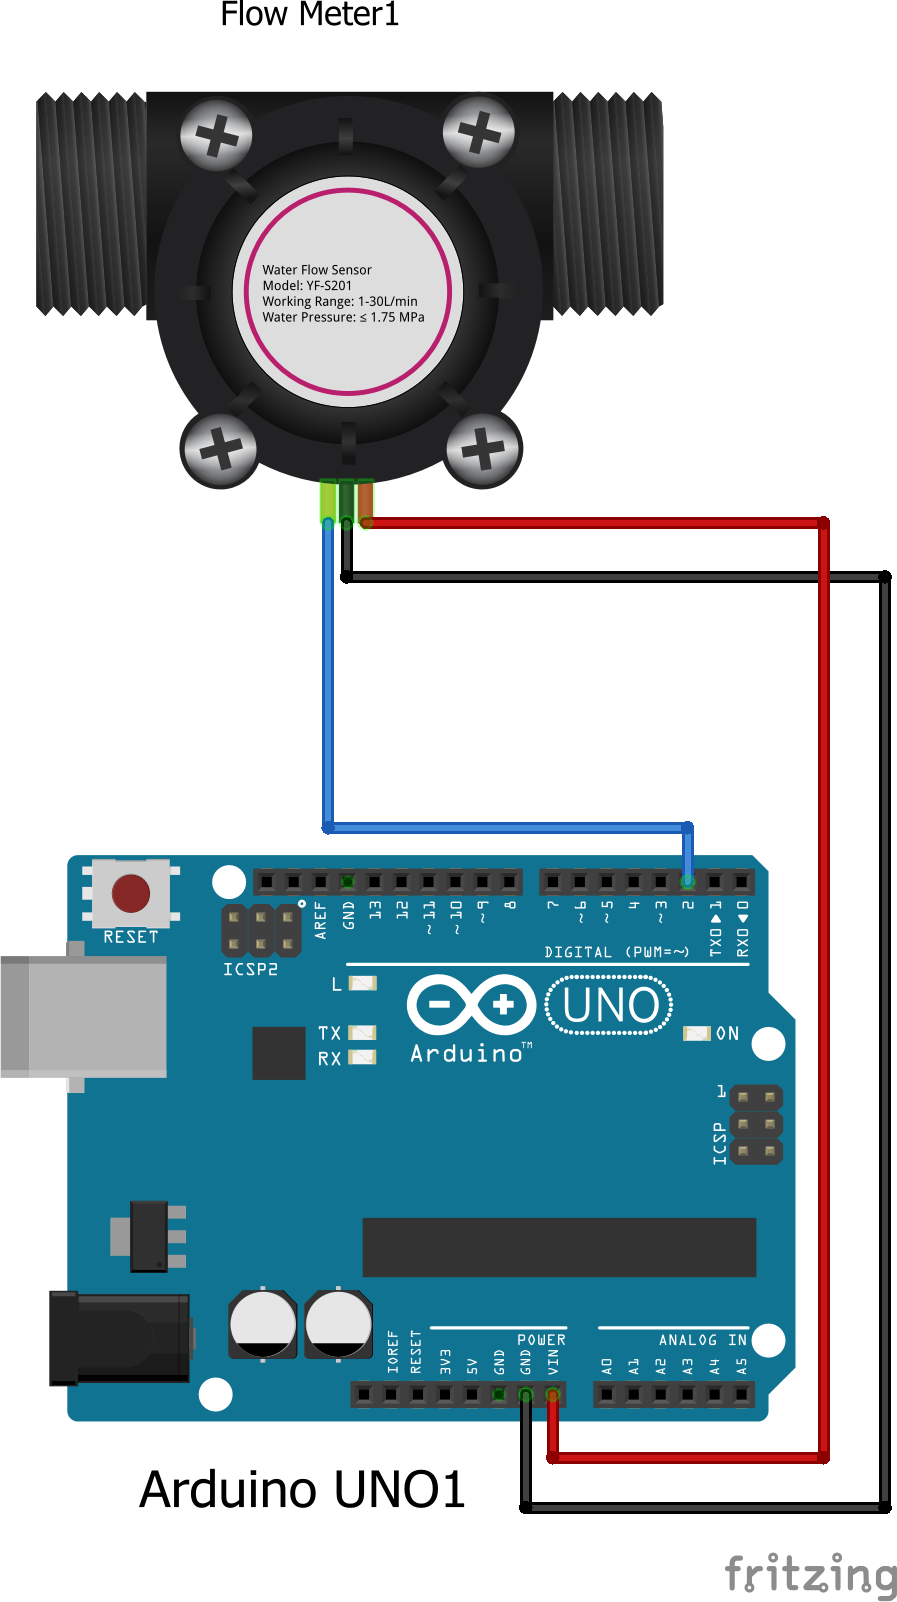
\includegraphics[width=0.5\textwidth]{figures/flow_bb.png}
\caption{Flow sensor to Arduino connection}
\label{FlowSensor}
\end{figure}
\subsubsection*{Interconnecting NodeMCU with Arduino}
Two Arduino can communicate to each other by universal asynchronous receiver transmitter(UART). Where one Arduino's Tx and Rx pin is connected to another one's Rx and Tx. Here Rx is for receive data and Tx is for transfer data. Transferring and receiving data is like master-slave relation. Arduino can send data to the wifi module asynchronously and NodeMCU can receive those data and if the internet is available it can through data to firebase real-time database.Figure \ref{NodeMCU} shows the connection between the Node MCU and arduino.
\begin{figure}[H]
\centering
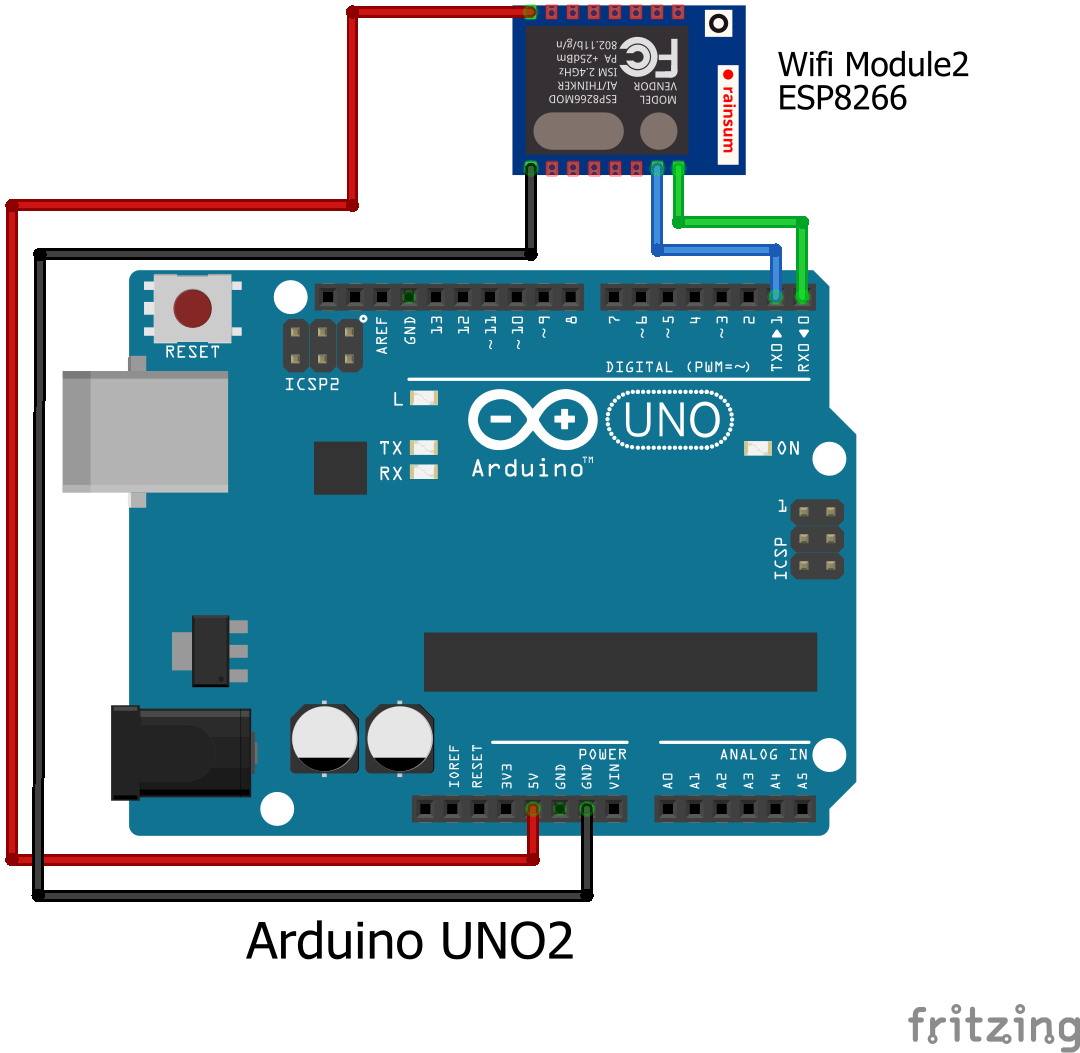
\includegraphics[width=0.5\textwidth]{figures/wifi_bb.png}
\caption{NodeMCU to Arduino connection}
\label{NodeMCU}
\end{figure}
\subsubsection*{Showing Data to Display}
A 16*2 liquid crystal display is used to showing sensor data. after receiving data from the Arduino wifi module display the data.Figure \ref{LCD} shows the connection between the LCD display and Node MCU.
\begin{figure}[H]
\centering
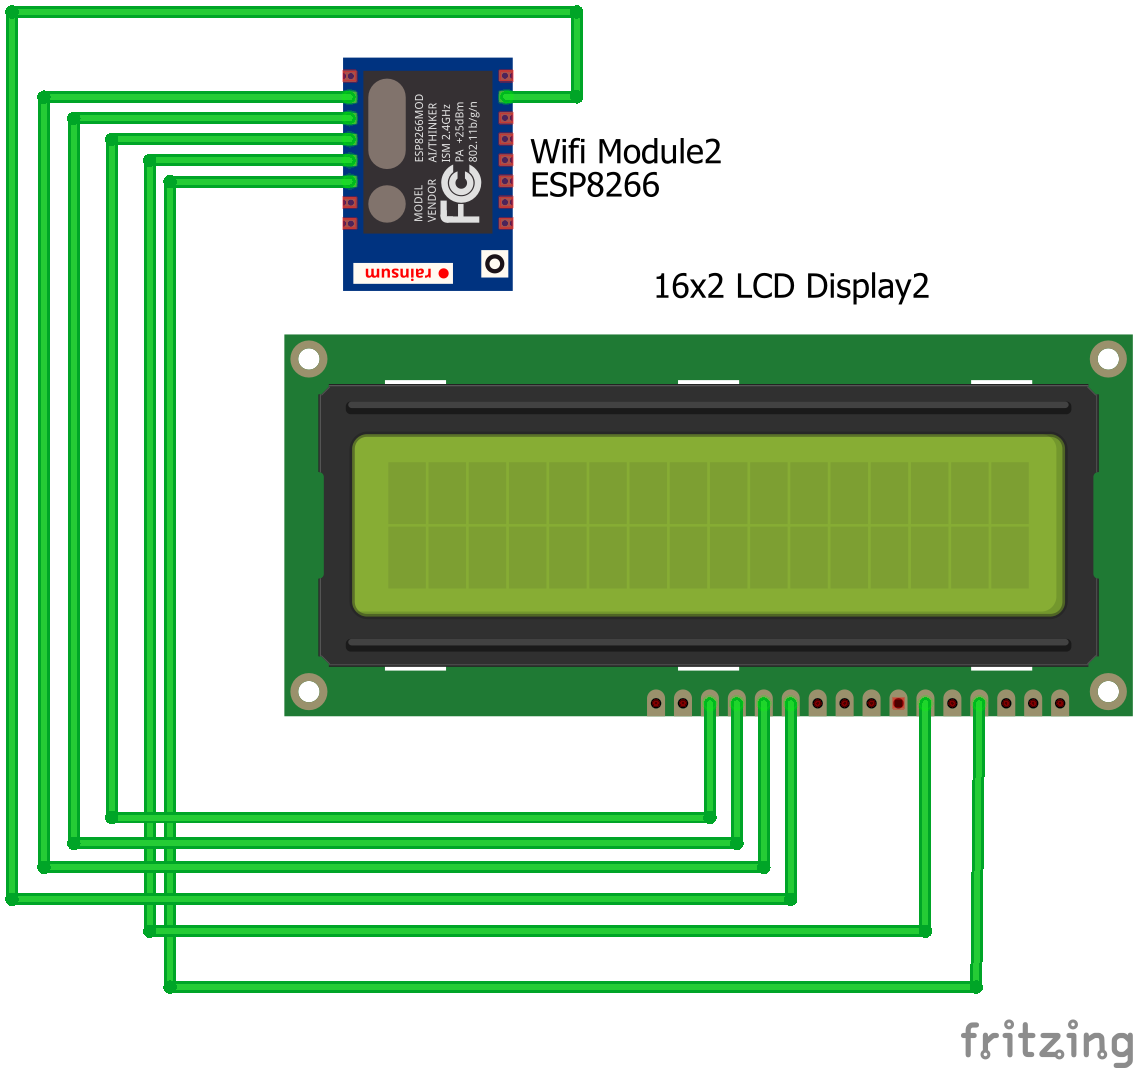
\includegraphics[width=0.5\textwidth]{figures/wifiDisplay_bb.png}
\caption{16*2 liquid crystal display to NodeMCU connection}
\label{LCD}
\end{figure}
\section{Implementation}
In this section, we will discuss the implementation procedure of our water quality monitoring and controlling system with more detail which is given below.

\subsection{Required Hardware }
% \item \textbf{Required hardware}
In our system, we used the following hardware components. In the following section, we discussed the application of these components to our project. We have selected these hardware components because they are comparatively cheaper than other chemical sensors. At experimental implementation, we can effectively find the feasibility of our proposed system using these components. 
\begin{itemize}
    \item[$-$] pH sensor 
    \item[$-$] Turbidity sensor
    \item[$-$] Ultrasonic sensor
    \item[$-$] Digital temperature sensor
    \item[$-$] Flow sensor
    \item[$-$] NodeMCU
    \item[$-$] Arduino UNO
    \item[$-$] GSM module
    \item[$-$] GPS module
    \item[$-$] Servo motor
    \item[$-$] Cleaning motor and brush
    \item[$-$] Display
    \item[$-$] Buzzer
    \item[$-$] Power adapter
\end{itemize}
\subsection{Required Software:}
\begin{itemize}
    \item[$-$] Arduino IDE
    \item[$-$] Android Studio
    \item[$-$] Google cloud server (Firebase)
    \item[$-$] Windows 10 Home
    \item[$-$] Water quality monitoring android application
\end{itemize}
\subsection{Required Programming Language:}
\begin{itemize}
    \item[$-$] Java
    \item[$-$] C
    \item[$-$] Extensive markup language (XML)
\end{itemize}

\subsection{Collecting water volume and use Water}
Figure \ref{filledTank} (a) shows a tank filled with water and figure \ref{filledTank} (b) shows that app is showing that the water has not been used.
\begin{figure}[H]
\centering
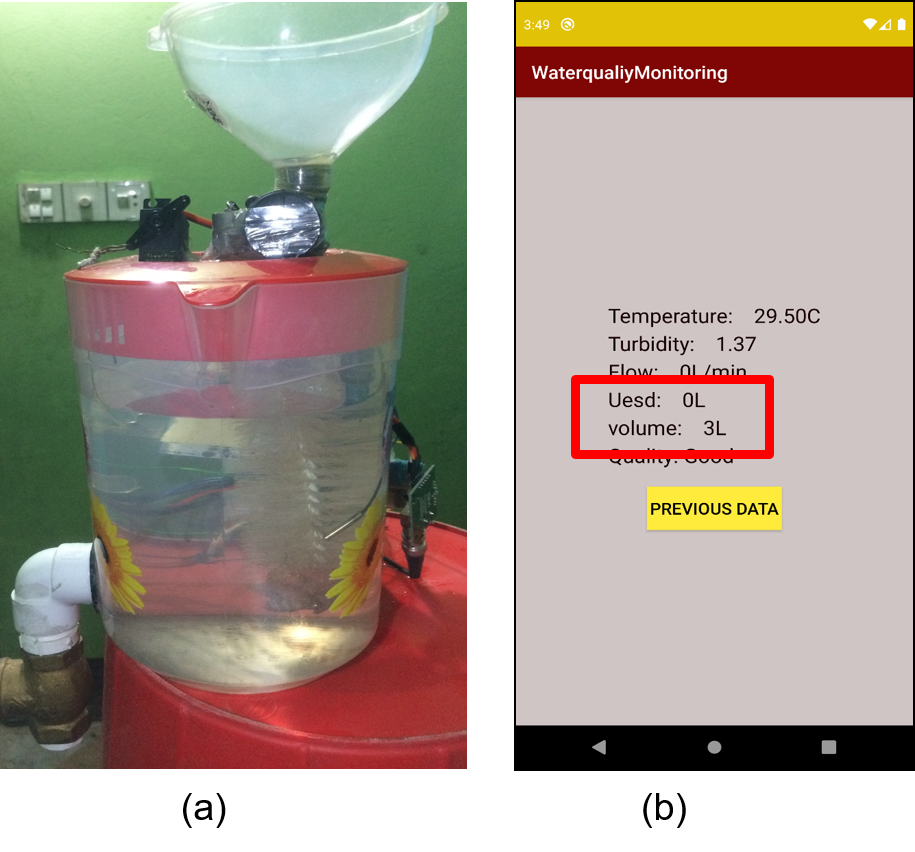
\includegraphics[width=0.5\textwidth]{figures/filledTank.png}
\caption{Tank status (a) tank filled with water (b) app shows no used water}
\label{filledTank}
\end{figure}
Figure \ref{emptyTank} (a) shows an empty tank and figure \ref{emptyTank} (b) shows that app is showing that the water has been used.
\begin{figure}[H]
\centering
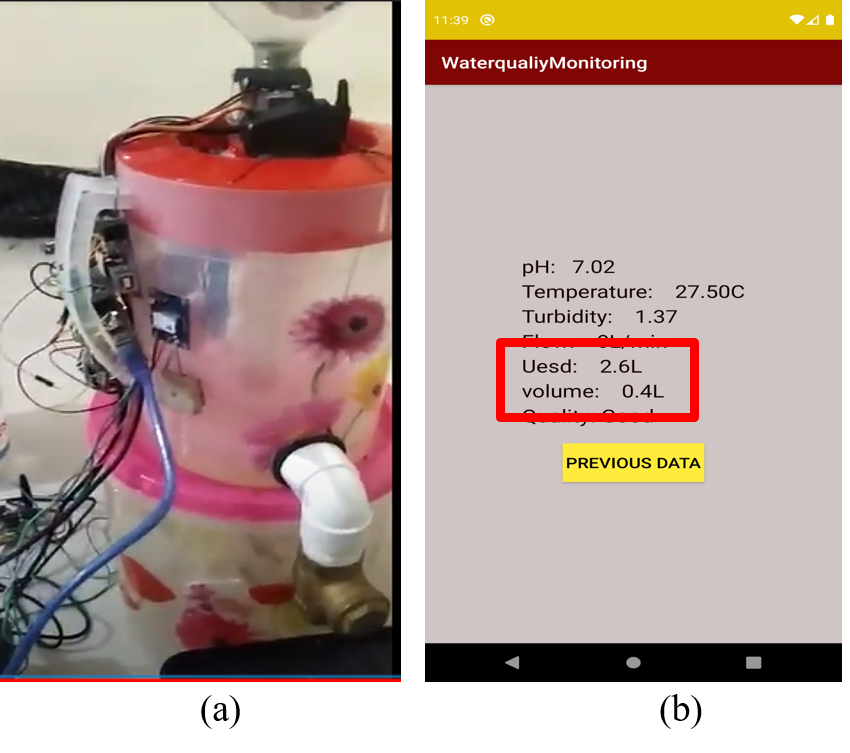
\includegraphics[width=0.5\textwidth]{figures/EmptyTank.png}
\caption{Tank status (a) empty tank (b) app show the used water is 2.6 L}
\label{emptyTank}
\end{figure}
\subsection{Cleaning and flushing tank}
The system check if the quality of the water is good or not. Figure \ref{cleanWater} (a) shows the tank full of clean water, \ref{cleanWater} (b) shows the result that the water quality is good.
\begin{figure}[h]
\centering
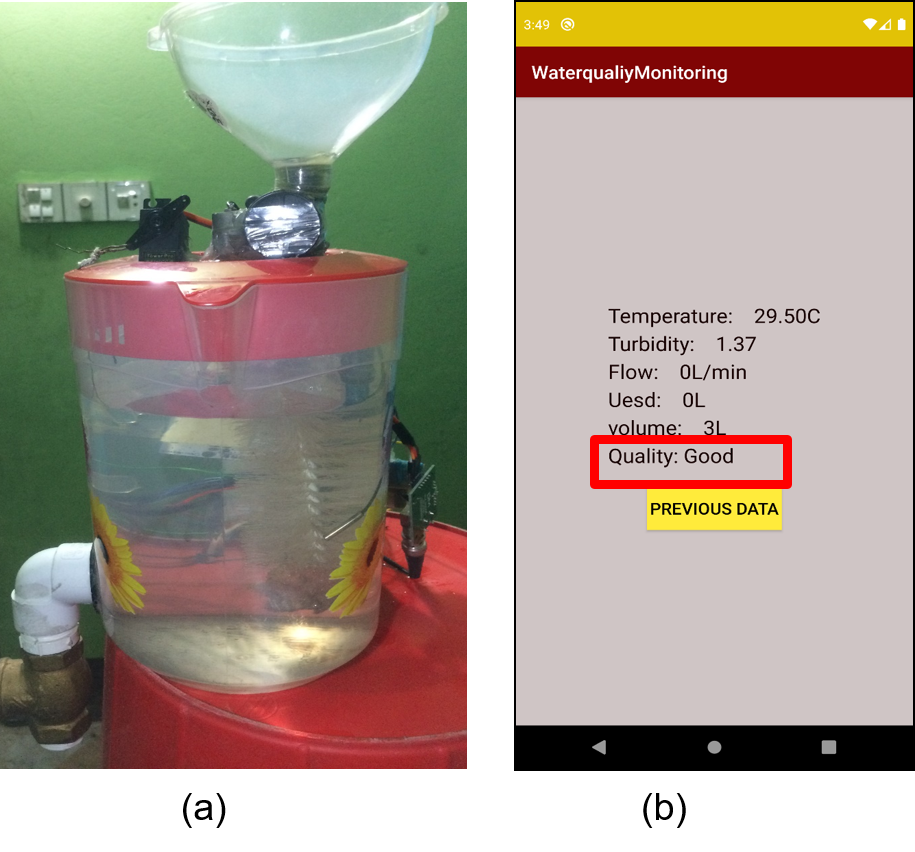
\includegraphics[width=0.5\textwidth]{figures/clearWater.png}
\caption{Water quality (a) clean water (b) app showing water quality good}
\label{cleanWater}
\end{figure}

Figure \ref{badWater} (a) shows the tank full of impure water, \ref{badWater} (b) shows the result that the water quality is bad.
\begin{figure}[h]
\centering
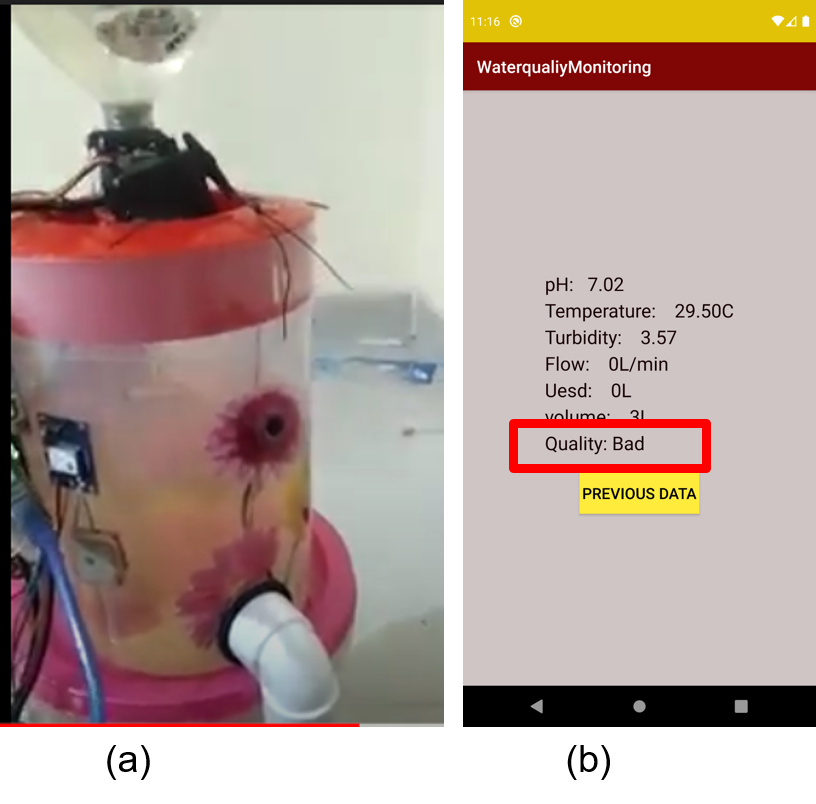
\includegraphics[width=0.5\textwidth]{figures/badWater.png}
\caption{Water quality (a) impure water (b) app showing water quality bad}
\label{badWater}
\end{figure}

After getting impure water the system starts rotate the brush installed inside the tank which is shown in figure \ref{flush} (a). Figure \ref{flush} (b) shows that the water is flushed out from the tank and figure \ref{flush} (c) shows the empty tank after the flush which means it is ready to fill again. 
\begin{figure}[h]
\centering
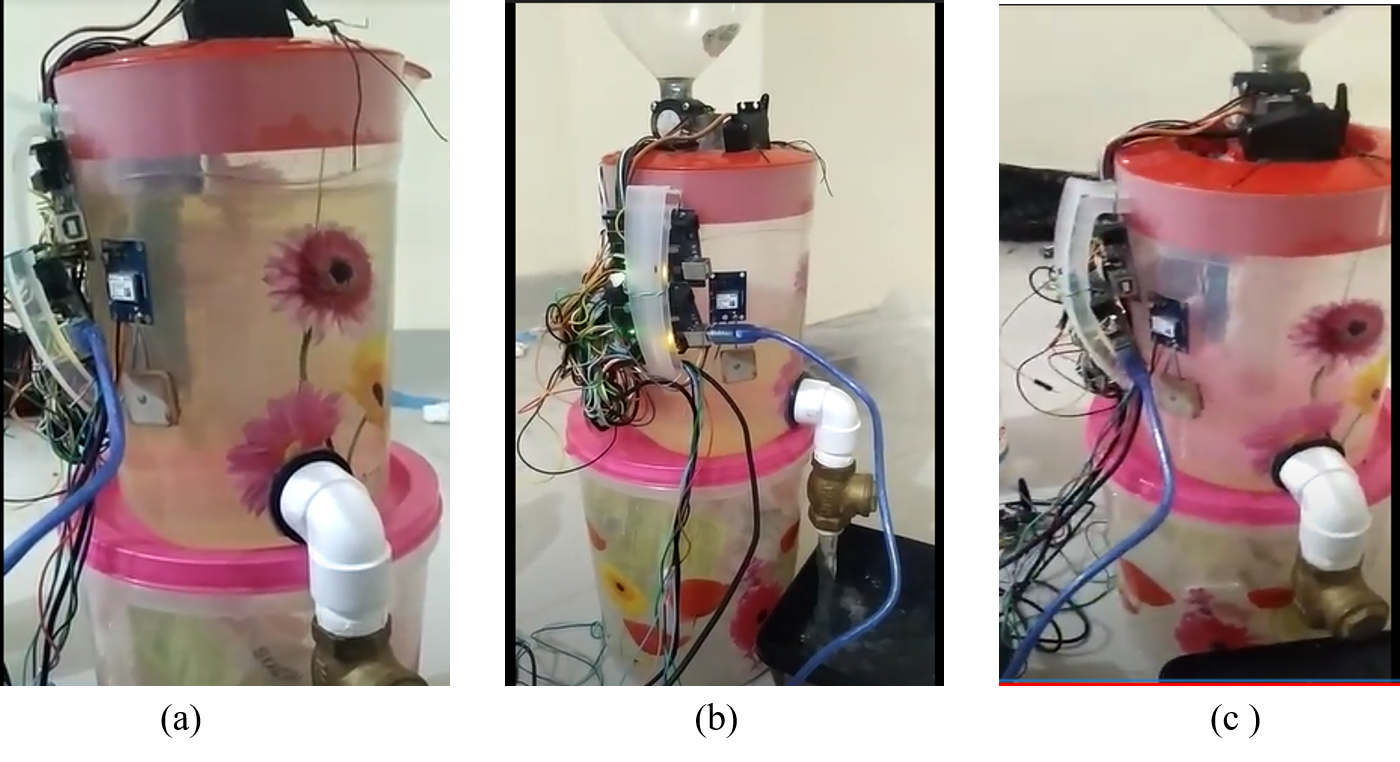
\includegraphics[width=0.8\textwidth]{figures/flush1.png}
\caption{Water quality (a) cleaning the tank (b) flushed (c) empty tank}
\label{flush}
\end{figure}
\subsection{Sending alert messages}
% \textcolor{red}{GIVE SOME DESCRIPTION LIKE THE ABOVE SECTION}
After calculating quality parameter data if water considered as impure water, A warning SMS with location is sent to tho respective person indicating that water gets dirty. And the geological location of the tank.
A screenshot image is given below.

\begin{figure}[H]
\centering
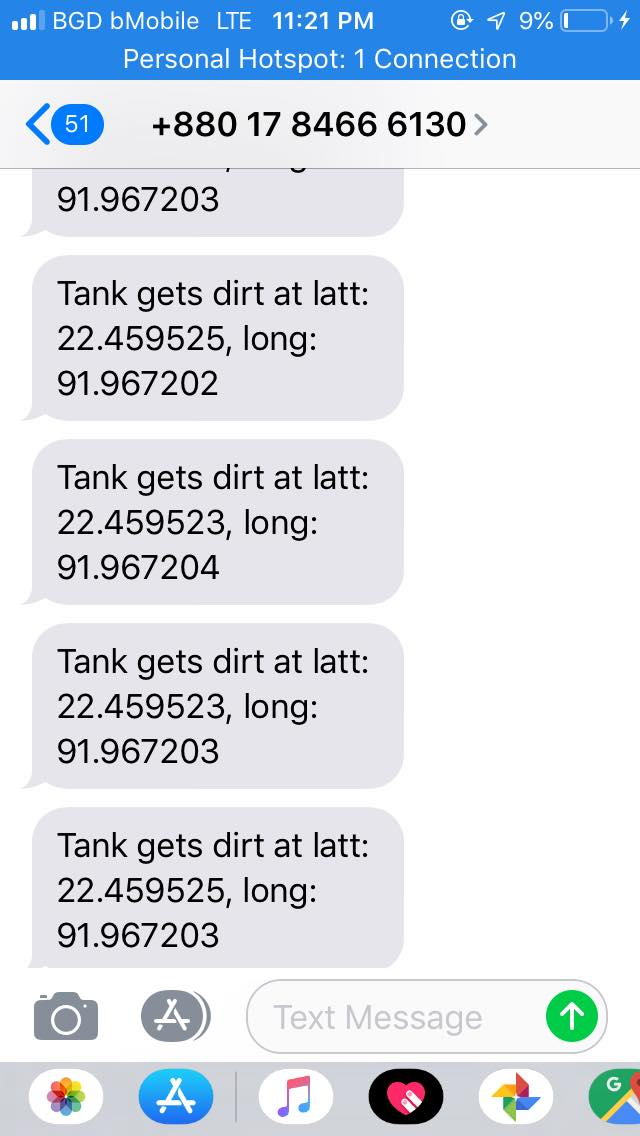
\includegraphics[width=0.5\textwidth]{figures/message.jpg}
\caption{Alert messages in mobile device}
\label{message}
\end{figure}
\section{Conclusion}
We explained how our designed system works in this section. The outline of the project structure is discussed. The required hardware components, software and programming languages are also discussed. We presented observations and discussions according to the approach.